%% LyX 1.6.5 created this file.  For more info, see http://www.lyx.org/.
%% Do not edit unless you really know what you are doing.
\documentclass[english]{article}
\usepackage[T1]{fontenc}
\usepackage[latin9]{inputenc}
\usepackage[letterpaper]{geometry}
\geometry{verbose,tmargin=1.1in,bmargin=1.1in,lmargin=1.1in,rmargin=1.1in}
\setlength{\parskip}{\medskipamount}
\setlength{\parindent}{0pt}
\usepackage{color}
\usepackage{verbatim}
\usepackage{graphicx}

\makeatletter

%%%%%%%%%%%%%%%%%%%%%%%%%%%%%% LyX specific LaTeX commands.
%% The greyedout annotation environment
\newenvironment{lyxgreyedout}{\textcolor[gray]{0.8}\bgroup}{\egroup}

%%%%%%%%%%%%%%%%%%%%%%%%%%%%%% Textclass specific LaTeX commands.
\newenvironment{lyxcode}
{\par\begin{list}{}{
\setlength{\rightmargin}{\leftmargin}
\setlength{\listparindent}{0pt}% needed for AMS classes
\raggedright
\setlength{\itemsep}{0pt}
\setlength{\parsep}{0pt}
\normalfont\ttfamily}%
 \item[]}
{\end{list}}

%%%%%%%%%%%%%%%%%%%%%%%%%%%%%% User specified LaTeX commands.
\linespread{1.2}

\makeatother

\usepackage{babel}

\begin{document}

\title{Optimization of Secure Function Evaluation\textit{\normalsize }\\
\textit{\normalsize Research Proposal for Ph.D Preliminary Exam}}


\author{Louis Kruger\\
University of Wisconsin Madison}

\maketitle
%
\begin{comment}
\tableofcontents{}
\end{comment}
{}


\chapter{Introduction}
\begin{quote}
%
\begin{comment}
\begin{quote}
As every man goes through life he fills in a number of forms for the
record, each containing a number of questions... There are thus hundreds
of little threads radiating from every man, millions of threads in
all. If these threads were suddenly to become visible, the whole sky
would look like a spider's web, and if they materialized as rubber
bands, buses; trams and even people would all lose the ability to
move, and the wind would be unable to carry torn-up newspapers or
autumn leaves along the streets of the city. They are not visible,
they are not material, but every man is constantly aware of their
existence.... Each man, permanently aware of his own invisible threads,
naturally develops a respect for the people who manipulate the threads.

--Alexander Solzhenitsyn, Cancer Ward, 1968.
\end{quote}

\end{comment}
{}
\end{quote}
Privacy and security are important concerns as computers increase
in power and the Internet continues to grow \cite{cra99,tur03}. Everyday
activities dealing with sensitive data are moving onto to the Internet,
such as credit card transactions, doctors accessing medical records,
and online banking. As a result, more data is stored on machines that
are connected to the Internet, directly or indirectly, then ever before.
Sadly, there are many all-too-common examples in the news of
privacy compromising activities such as phishing, data theft, and
identity theft. New techniques are needed to deal with the many threats
to privacy. In addition to the misuse of data, there can be other
consequences of privacy violations, such as serious legal penalties
for violation of HIPAA laws \cite{hippa}, which mandate strict privacy
requirements among health-care professionals.

Despite these many privacy concerns, there is also a conflicting desire
to perform useful computations with sensitive data. Data is not useful
unless it can be accessed and manipulated. Sometimes various parties
would like to collaborate on research involving this data. For
example, genetic data is the subject of much current research, but
it is considered private personal information. Researchers with access
to different patients' data may want to combine their information
resources in the search for new cures for diseases, without revealing
the actual sensitive information to the collaborating parties. Competing
businesses may want to jointly perform market research for mutual
benefit, without exposing their sensitive business data. Therefore,
the challenge
is how to balance these competing concerns, making data available
for desirable uses while preserving as much privacy as possible.  By
providing strong privacy guarentees, we enable new uses of sensitive data.

These concerns are not merely theoretical. In 2000, Ford Motor Explorer
SUVs had a well publicized problem with their Firestone tires, in
which the tire treads could fail under certain circumstances. At least
271 deaths resulted \cite{NYTFordFirestone}. The problem resulted
from the \emph{combination} of products: There were no problems with
the same tires in other vehicles, nor with Ford Explorers using other
tires. It has been suggested that the crisis could have been averted
using joint data-mining, however, due to business secrecy concerns,
such research could only have been done using privacy preserving methods
\cite{VaidyaClifton:2002}.

There have been several methods developed so far for preserving personal
privacy while permitting use of data. The most simple method, conceptually,
is to replace identifying information, such as the name, social security
number, and other sensitive data with random unique identifiers, and
then using the transformed data for computation. If it is necessary
to correlate the outputs of the computation with individuals, the
data owner can do this, but other parties presumably can not. However,
this method has been shown to be vulnerable to attacks that correlate
the transformed data with information available from external sources
to reconstruct the obfuscated data, thereby breaking the privacy protection
\cite{Malin04}. 

Another method for preserving privacy is known as \emph{secure multiparty
computation}\cite{Yao86}. This is a technique of performing computations on inputs
supplied by multiple parties while provably maintaining privacy guarantees.
If the computation is a function evaluation, then it is called \emph{secure
function evaluation}, or SFE. This is a technique which in theory can address
many of the privacy concerns we face. The inputs to
the function are partitioned among more than one party, and the function
is computed collaboratively while preserving the privacy of each participant's
individual inputs. In this case, privacy is considered preserved if
no party learns any information that would affect their estimate of
the probability distribution of another party's inputs, except for
that which can be calculated by the parties' own inputs and the output
of the joint function. In comparison with other methods, only secure
multiparty computation can be used to guarantee privacy when parties
collaborate on joint computation. %
\begin{comment}
%
\begin{lyxgreyedout}
Needs clarification
\end{lyxgreyedout}
 In other words, the entropy gain of each party is equivalent to the
entropy gain in an idealized protocol where a trusted third party
collects all the inputs, evaluates the function, and transmits only
the output to each party. Depending on the protocol, the guarantees
for some parties may be based on typical assumptions of computational
hardness, while the guarantees for other parties may be information
theoretic.
\end{comment}
{}

Although SFE has provable privacy guarantees, its implementation tends
to be very expensive for practical use in terms of time and space.
The space expense manifests itself in the large consumption of network
bandwidth used in the protocols, and the time expense comes from repeated
use of expensive cryptographic primitives, such as modular exponentiation.
These expenses explain why SFE has not been frequently used outside
of the academic literature, despite the fact that it was formally
introduced in the literature in the early 1980s \cite{Y82}. There has
been research in recent years to make SFE more practical. This research
falls into two categories: general and function specific. General
protocols allow any function expressed as a circuit computation to
be evaluated securely. The Fairplay system \cite{Fairplay} is a straightforward
implementation of the Yao protocol \cite{Yao86}, presented in section
\ref{sub:Garbled-Circuit-Method}, along with a supporting compiler
that allows secure functions to be written in a more familiar functional
programming notation. We showed
how \emph{Ordered Binary Decision Diagrams} (OBDD)  can be used to
produce a more efficient protocol for secure evaluation for certain
functions\cite{kruger06}. Function specific protocol design has produced secure protocols
which perform dramatically better than general protocols. Privacy-preserving data mining (PPDM) has been a major application driving
such research \cite{verykios04stateart}. Other protocols have been
developed for various classes of functions such as polynomial evaluation
\cite{naor99otope} and string alignment algorithms such as edit distance
\cite{kruger07}.  Moore's law has been a factor as well which benefits privacy-preserving protocols.
We have shown that in many
cases, the computation requirements of general protocols
can be adequate for practical use when performed on modern
CPUs \cite{kruger06,kruger10}.

We have researched ways to improve the efficiency and practicality
of privacy preserving protocols. Our work has investigated finding
efficient protocols for specific classes of functions; for example
one study analyzes several designs of a $k$-means clustering algorithm
\cite{kruger05}, and another discusses ways to design efficient protocols
for many kinds of dynamic programming problems \cite{kruger07}. We
have also investigated the use of alternate circuit representations
using OBDDs to improve the performance of general purpose protocols
and showed that they can be beneficial for certain functions \cite{kruger06}.
These works are discussed in section \ref{sec:Techniques}.
We also demonstrated a practical application of SFE as a new approach
to solving classic security problems with password authentication, using
SFE to model the hashing functions used in traditional password schemes.
\cite{kruger10}

Our thesis statement is this:  SFE can be used for practical purposes today,
enabling privacy-preserving computation to thrive in today's distributed
world. In the rest of this document, we will demonstrate this thesis through
practical examples of the use of SFE.  We will show how traditional algorithms
can be adapted to preserve privacy, such as in the case of K-means clustering
and privacy preserving genomic algorithms.  We will show how cryptographic
primitives suitable for real-time use can be developed by presenting an
oblivious transfer protocol based on the modular square roots.  We will
also show how traditional security problems can be solved using SFE,
by presenting a secure protocol for password authentication with strong
security guarentees and legacy interoperability that is better than other
authentication protocols in common use.




\section{Background and Related Work}


\subsection{Primitives \label{sub:Primitives}}


\subsubsection{Oblivious Transfer}

Oblivious transfer is a protocol originally proposed by Rabin \cite{Rabin81}.
Informally, a 1-out-of-n oblivious transfer, denoted as $OT_{n}^{1}$,
is a protocol between two parties, the Chooser and the Sender. The
Sender's inputs into the protocol are $n$ values $v_{1},...,v_{n}$.
The Chooser's input is an index $i$ such that $1\le i\le n$. As
a result of the protocol, the Chooser receives $v_{i}$, but does
not learn any additional information about the rest of the Sender's
values. The Sender learns nothing. 

The Naor-Pinkas OT protocol \cite{NaorPinkas99}, based on discrete
logarithms, is considered to be the most efficient OT protocol for
practical use today. The performance characteristics of this protocol
are discussed in section \ref{sub:Comparison-with-Naor-Pinkas}.


\subsubsection{Homomorphic Encryption}

Homomorphic Encryption is a class of public key encryption algorithms
that satisfies a homomorphism property. An additive homomorphic cipher
satisfies $E(a+b)=E(a)\oplus E(b)$ where $\oplus$ is an efficiently
computable operator that requires no secret information. Similarly,
a multiplicative homomorphic cipher satisfies $E(ab)=E(a)\otimes E(b)$.
Some of the most famous public key ciphers have the multiplicative
homomorphic property, including the Elgamal cipher \cite{elgamal85}
and the RSA cipher \cite{rivest83rsa}. The homomorphic properties
have traditionally been considered undesirable for general purpose
cryptography \cite{jmsw02}. %
\begin{comment}
mention Cramer-Shoup?
\end{comment}
{}Specifically, the malleability of ciphertexts can allow the adversary
to violate integrity constraints, and also make such ciphers insecure
against %
\begin{comment}
 because the homomorphic structure aids in cryptanalysis and allows
encrypted messages to be modified, violating integrity constraints.
\cite{jmsw02}. This leads to insecurity against
\end{comment}
{}\emph{adaptive chosen ciphertext} (CCA2) attacks \cite{bleichenbacher98chosen}.
However, homomorphic encryption schemes have also found use in novel
cryptographic applications such as secure voting \cite{benaloh94}. 
\begin{description}
\item [{Semantically~secure~additive~homomorphic~encryption.}] This
is a cipher which satisfies certain properties that are useful in
SFE protocols. Let $(G,E,D,M)$ be a public-key encryption scheme.
$E_{e}(m)$ and $D_{d}(c)$ are the encryption and decryption functions
for plaintext $m$ and ciphertext $c$, with respect to a public/private
key pair ($e,d)$. $G$ is a key generation function that can be used
to randomly generate $(e,d)$ pairs, and $M$ is the message space
respectively. \end{description}
\begin{itemize}
\item The encryption scheme is semantically secure \cite{Goldwasser:Micali}.
Informally, this means that the ciphertext leaks no useful information
about the plaintext even if the attacker has previously observed many
plaintext-ciphertext pairs on plaintexts of his choice. Formally,
let $P(m)$ be any efficently computable Boolean predicate $P(m)$.
WLOG, assume that $Pr[P(m)\mbox{ is true}]=p\ge0.5$ if $m$ is chosen
uniformly from $M$. For any $m$, the adversary, given $E(m)$ must
not be able to correctly compute $P(m)$ with probability $p+\epsilon$,
unless $\epsilon$ is negligible. With any semantically secure encryption
scheme, encrypting the same message twice will yield different ciphertexts
with high probability, so $E(m)$ must be a randomized one-to-many
function representing a set of possible ciphertexts that can be obtained
by encrypting $m$. Naturally, if $m_{1}\neq m_{2}$, then $E(m_{1})\cap E(m_{2})=\emptyset$
\item There exists a computable function $f$, computable without the private
key or other secret information, such that for all messages $m_{1}$,
$m_{2}$, and $c_{1}\in E(m_{1})$, $c_{2}\in E(m_{2})$, the following
property holds:\\
$f\left(c_{1},c_{2}\right)\in E(m_{1}+m_{2})$
\item There exists a computable function $g$ such that for all $m_{1}\in M$
and $\alpha\in M$, $c_{1}\in E(m)$ implies that $g(c_{1},\alpha)\in E(\alpha m_{1})$.
In addition, $g$ must be computable without using the private key
or other secret information. This property follows automatically from
the previous requirement, because it is always possible to define
$g$ in terms of $O(\log\alpha)$ invocations of the function $f$.
\end{itemize}
There are several encryption schemes that satisfy these properties,
of which Paillier's encryption scheme, based on composite residue
classes, is the most widely used \cite{Paillier99}. In the Paillier
cryptosystem, the message space is $m<n$, where $n=pq$ for $p$
and $q$ prime. The ciphertext space is $E(m)<n^{2}$. Let $g<n^{2}$
such that $g$ has order $n\alpha$. Using the public key $(g,n)$,
the encryption function $E(m)=g^{m}r^{n}\left(\mbox{mod }n^{2}\right)$,
for a random $r<n$. Using the private key $\lambda=\mbox{lcm}(p-1,q-1)$,
the decryption function for ciphertext $c$ is $m=\frac{L\left(c^{\lambda}\mbox{ mod }n^{2}\right)}{L\left(g^{\lambda}\mbox{ mod }n^{2}\right)}\mbox{ mod }n$
where $L(u)=\frac{u-1}{n}$ is a well defined function for $u\equiv1\;(\mbox{mod }n)$.
Notice that $E(m_{1})\cdot E(m_{2})=g^{m_{1}}r_{1}^{n}g^{m_{2}}r_{2}^{n}=g^{m_{1}+m_{2}}(r_{1}r_{2})^{n}\in E(m_{1}+m_{2})$,
which satisfies the additive homomorphic property. Further details
can be found in \cite{Paillier99}.


\subsection{Secure Function Evaluation}

One of the fundamental cryptographic primitives for designing privacy-preserving
protocols is \textit{secure function evaluation (SFE)}. A protocol
for SFE enables two parties $A$ and $B$ with inputs $x$ and $y$
respectively to jointly compute a function $f(x,y)$ while preserving
the privacy of the two parties' respective inputs. At the end of the
protocol, party $A$ only knows its input $x$ and the value of the
function $f(x,y)$, and a similar condition holds for $B$. It was
proved by Yao \cite{Yao86} and Goldreich, Micali, and Wigderson \cite{GMW87}
that for a polynomially computable function $f$, there exists protocols
for securely evaluating $f$ that executes in polynomial time. Both
proofs are constructive, and provide a method for transforming a Boolean
circuit description of the function $f$ into a protocol for secure
evaluation of $f$. These protocols are summarized here.


\subsubsection{Garbled Circuit Method \label{sub:Garbled-Circuit-Method}}

Consider any Boolean circuit $C$, and two parties, Alice and Bob,
who wish to evaluate $C$ on their respective inputs $x$ and $y$.
In Yao's {}``garbled circuits'' method \cite{Yao86}, Alice securely
transforms the circuit so that Bob can evaluate it obliviously, i.e.,
without learning Alice's inputs or the values on any internal circuit
wire except the output wires. The steps are as follows:
\begin{enumerate}
\item Alice generates two random keys $k_{i,0}$ and $k_{i,1}$ for each
circuit wire $i$, one representing $0$ on that wire, the other representing
$1$. For all wires in the circuit except input wires, the truth table
for the corresponding Boolean gate is encrypted. If $g(x,y)$ is a
gate with input wires $j$ and $l$, and output wire $i$, then the
truth table value for $g(x,y)$ is encoded as $E_{k_{j,x}}\left(E_{k_{l,y}}\left(k_{i,g(x,y)}\right)\right)$.
Here, $k_{j,x}$ is the encryption key for value $x$ of wire $j$,
and similarly for $k_{l,j}$. $k_{i,g(x,y)}$ is the encryption key
for the output wire of $g$ with value $g(x,y)$ The four encrypted
values representing $g(0,0)$, $g(0,1)$, $g(1,0)$, and $g(1,1)$
fully specify the gate $g$. Alice sends the garbled circuit to Bob.
Computation of the garbled circuit does not depend on input values
and can be performed in advance. However, the same garbled circuit
must not be used more than once, or Alice's privacy may be violated.
\item Alice sends the keys corresponding to her own input wires to Bob.
Bob obtains the keys corresponding to his input wires from Alice using
an $OT_{2}^{1}$ protocol. For each of Bob's input wires, Bob acts
as the chooser using his circuit input bit as his input into $OT_{2}^{1}$
, and Alice acts as the sender with the two wire keys for that wire
as her inputs into $OT_{2}^{1}$ .
\item Bob evaluates the circuit. Because of the way that the garbled circuit
is constructed, Bob, having one wire key for each gate input, can
decrypt exactly one row of the garbled truth table and obtain the
key encoding the value of the output wire. Yao's protocol maintains
the invariant that for every circuit wire, Bob learns exactly one
wire key. Because wire keys are random and the mapping from wire keys
to values is not known to Bob (except for the wire keys corresponding
to his own inputs), this does not leak any information about actual
wire values. The circuit can thus be evaluated obliviously. A complete
description of Yao's method and security proofs can be found in \cite{Goldreich:vol2}.
\end{enumerate}

\subsubsection{Secure Computation With Random Shares}

\cite{GMW87} presents a protocol for securely evaluating circuits
known as \emph{secure computation with shares} (SCWS). This protocol
maintains the invariant that, for every circuit wire $w$, Alice learns
a random value $s$ and Bob learns $b_{w}\oplus s$, where $b_{w}$
is the bit value of the wire. Therefore, Alice's and Bob's shares
add up to $b_{w}$, but because the shares are random, neither party
knows the actual wire value. For each output wire of the circuit,
Alice and Bob combine their shares to reconstruct the circuit output.
Suppose $g(x,y)$ is a gate, $x$ and $y$ are the input wires to
the $g$ and $x_{a}\oplus x_{b}=x$ and $y_{a}\oplus y_{b}=y$ are
Alice and Bob's shares of $x$ and $y$. The following steps will
securely evaluate the gate:
\begin{enumerate}
\item Alice selects a random bit $z_{a}$ 
\item Alice constructs a quadruple $\left(g(x_{a},y_{a})\oplus z_{a},\, g(x_{a},1-y_{a})\oplus z_{a},\, g(1-x_{a},y_{a})\oplus z_{a},\, g(1-x_{a},1-y_{a})\oplus z_{a}\right)$. 
\item Using an $OT_{4}^{1}$ protocol, Bob selects the bit from Alice's
quadruple with index $s=2x_{b}+y_{b}$. The value received by Bob
is $z_{b}=g(x_{a}\oplus x_{b},y_{a}\oplus y_{b})\oplus z_{a}=g(x,y)\oplus z_{a}$. 
\end{enumerate}
At the beginning of the evaluation, Alice sets her share of the input
wires to her input values, and her share of Bob's input wires to $0$,
and vice versa for Bob. Each gate $g$ may be evaluated after Alice
and Bob have computed their shares of the gate's input wires. Thus,
by repeated applying the above steps, the entire circuit can be evaluated
starting from the inputs, and progressing gate by gate until the output.
Further details and security proofs are presented in \cite{Goldreich:vol2}.

In practice, the garbled circuit method is more commonly used, because
it is more efficient. Then garbled circuit method requires only a
single transfer of data from Alice to Bob, followed by an $OT_{2}^{1}$
for each the $|B|$ values representing Bob's inputs. These OTs can
be combined into a single parallel OT. Then Bob obliviously evaluates
the entire circuit on his own, and sends the output keys of Alice's
outputs back to her. In contrast, the SCWS method requires an $OT_{4}^{1}$
for each gate. This will require at least $depth(C)$ distinct rounds
of the OT, where $depth(C)$ is the maximum number of gates along
any path from an input to an output. The increased number of OTs,
combined with the increased number of rounds needed to execute them,
makes the SCWS evaluation protocol primarily of theoretical interest.
However, the SCWS principle can be emulated with the Yao protocol,
by explicitly including extra gates in the circuit to combine and
split the share values. 


\subsection{Implementations}

In recent years, there have been implementations of SFE undertaken
by researchers to design secure multiparty protocols. In the past,
SFE was considered a theoretical topic too expensive for practical
use, but the convergence of ubiquitous communication using the Internet,
more efficient cryptographic primitives, and the exponentially increasing
availability of processing power and network bandwidth are making
SFE an area of increasingly significant practical value.


\subsubsection{Fairplay}

Fairplay \cite{Fairplay} is an example of an SFE implementation designed
to enable wider application of SFE. Fairplay is the first system,
designed to be practical, that attempts to make SFE using Yao's protocol
available to a wider audience. It consists of a compiler that takes
as input a function $f$ defined using a procedural language called
\emph{Secure Function Description Language} (SFDL), and outputs a
Boolean circuit to evaluate $f$ using a description language called
\emph{Secure Hardware Description Language} (SHDL). Fairplay also
includes an implementation of the two party Yao protocol which securely
evaluates an SHDL function. \cite{Fairplay} provides the first empirical
measurements from an implementation of the Yao protocol.


\subsubsection{Application specific}

Fairplay showed that the classic protocol for SFE is still quite expensive
for all but the simplest circuits. There has been much research effort
in designing more efficient privacy-preserving protocols for many
problems of interest. In \cite{Reiter:CCS:2003}, a compiler was implemented
for generating secure two-party protocols for a restricted class of
functions built from modular arithmetic. The particular design was
motivated by the desire to build efficient secure protocols such as
signature schemes and threshold cryptography. Secure protocols have
been implemented for many problems such as auctions \cite{NPS99},
set intersection \cite{FNP04}, and conducting surveys \cite{FNP04}.
A particularly important application of secure computation is discussed
in the next section.


\subsection{Privacy Preserving Data Mining }

Initial focus in this area was on construction of decision trees from
distributed data sets \cite{Agrawal-Srikant,Lindell-Pinkas}. There
is also a significant body of research on privacy-preserving mining
of association rules \cite{Gehrke:2002,RizviHarista,VaidyaClifton:2002}.
In general, there are two approaches for designing privacy-preserving
data mining algorithms. The first approach is to use transformations
to perturb the data set before the algorithm is applied, by replacing
sensitive data with random unique identifiers. This approach for designing
privacy-preserving algorithms is taken by several researchers \cite{Klusch,MeruguGhosh,Oliveira}.
However, this approach suffers from the lack of formal security guarantee,
and has been shown to be vulnerable to data correlation attacks \cite{Malin04}.
Secure multiparty computation is the basis of the other approach.
A survey of such techniques is presented in \cite{PinkasCryptoPPDM02}.
This approach is the primary topic discussed here.

\subsection{Password Authentication}
Password authentication is a well-known means for accessing services as a user with a known
identity.

\subsection{Threat Models\label{sub:Threat-Models}}

In the {}``semi-honest'' threat model, also known as {}``honest
but curious'', or {}``passive'', a party to the computation is
assumed to behave correctly and follow the protocol as prescribed.
However, the party also runs additional probabilistic polynomially
bounded computation on the side in order to learn information to which
he is not entitled. A security proof using the semi-honest threat
model implies that the protocol as designed does not {}``leak''
information. The semi-honest model is an important theoretical tool
despite the fact that it is weaker and does not capture the full range
of malicious behaviors we would expect of an adversary. This is because
a protocol that has been proven secure in the semi-honest model can
be extended in an automated way, using a protocol {}``compiler'',
to a more secure protocol that is secure in the malicious model \cite{GMW87}.
Essentially, the protcol compiler inserts additional steps into the
protocol to force the parties to prove to one another their faithful
adherence to the protocol. The semi-honest model may itself be a realistic
model in certain cases, for example, when the parties communicating
need to preserve privacy of data from one another, but also have a
sufficient trust relationship not to intentionally cheat.

In the {}``malicious'' threat model, a badly behaving party is free
to use any available methods to thwart the computation , including
sending false or inconsistent messages at any step of the protocol.
The malicious threat model naturally characterizes the malicious behavior
that a secure protocol would need to protect against. If a protocol
is shown to be secure in the malicious threat model, then we can reasonably
assume that a malicious party or interloper will not be able to learn
any private information by attacking the protocol.

In the {}``covert'' threat model, similar to the {}``malicious'' model,
a badly behaving party is free to use any available methods to thwart the computation.
Although the allowable behavior of the adversary is the same, the security
guarentee is relaxed.  In particular, a protocol is considered secure
in the covert model if the probability of the attacker not getting caught
is small but non-negligable.  The covert model can be considered appropriate
for real-world scenarios only when the consequences to the adversary for being
caught are a significant deterrence to trying to cheat (i.e. loss of reputation,
monetary or legal penalties, etc) compared to the benefit of a successful attack.
\cite{aumannlindell}

%
\begin{comment}
\bibliographystyle{plain}
\bibliography{privacy,somesh,crypto}

\end{comment}
{}



\chapter{Techniques for Protocol Optimization}

\label{sec:Techniques}

Optimizing secure function evaluation to make it more practical for
real world use will be the focus of this thesis. Traditional methods
for SFE, such as Yao's secure circuit evaluation protocol \cite{Yao86},
are many orders of magnitude slower than the straightforward insecure
evaluation of functions, with factors of thousands or more. Asymtotically,
the time required to perform secure function evaluation is equivalent
to the time required to execute the function itself. For example,
the Yao protocol requires time and communication linear in the number
of circuit gates. However, the need to encrypt every gate with multiple
keys, and to perform oblivious transfer on every circuit input is
the cause of the enormous slowdowns. These tremendous performance
penalties in the generic constructions highlight the need for optimizing
SFE.

There are various ways to approach the problem of designing optimized
secure function evaluation protocols. This thesis focuses on three
general methodologies. From most specific to most general, three approaches
we have looked at are algorithm specific, algorithm \emph{class} specific,
and a general approach that is applicable to all computable functions.
The trade-off between these different approaches is a balance between
performance and general applicability. This trade-off has an analogy
in the literature of programming language compiler optimizations.
General code optimizations, such as loop-unrolling or strength-reduction
can make all code faster to a limited degree (although this is not
guaranteed), but tuning a specific algorithm by hand often yields
superior results. Algorithm class methods fall in between, with conceptual
ideas that apply to classes of algorithms related by design methodology,
such as dynamic programming problems.


\section{General: Protocol Optimization using Ordered Binary Decision Diagrams}

\label{OBDD-section}

In this work, we evaluated the use of alternate representation of
Boolean circuits as a way to create more efficient general purpose
secure function evaluation protocols. An \emph{Ordered Binary Decision
Diagram} (OBDD) is a directed acyclic graph-based representation of
a Boolean function that has been used in a variety of applications
in computer-aided design, including symbolic model checking (a technique
for verifying designs), verification of combinational logic, and verification
of finite-state concurrent systems \cite{Bryant:BDD,Clarke:book}.
OBDDs can be readily extended to represent functions with arbitrary
domains and ranges. An OBDD is similar to a decision tree, in that
evaluation is performed from a head node to leaves. However, an OBDD
is not ordinarily a tree, because internal nodes with identical structure
are shared. Given a function $f(x_{1},x_{2},\cdots,x_{n})$, the OBDD
for that function will have $n$ levels, with the $i^{th}$ level
corresponding to variable $x_{l_{i}}$, where $(l_{1},\cdots,l_{n})$
is a permutation of $(1,\cdots,n)$. There is a unique canonical OBDD
corresponding to any function with respect to a given ordering $(l_{1},\cdots,l_{n})$.
An example of an OBDD to compute the function $F(x)=\#x1\#x3>\#x2\#x4$
(two-bit millionaires' problem) is shown in \ref{fig:OBDD-example}.

%
\begin{figure}
\begin{centering}
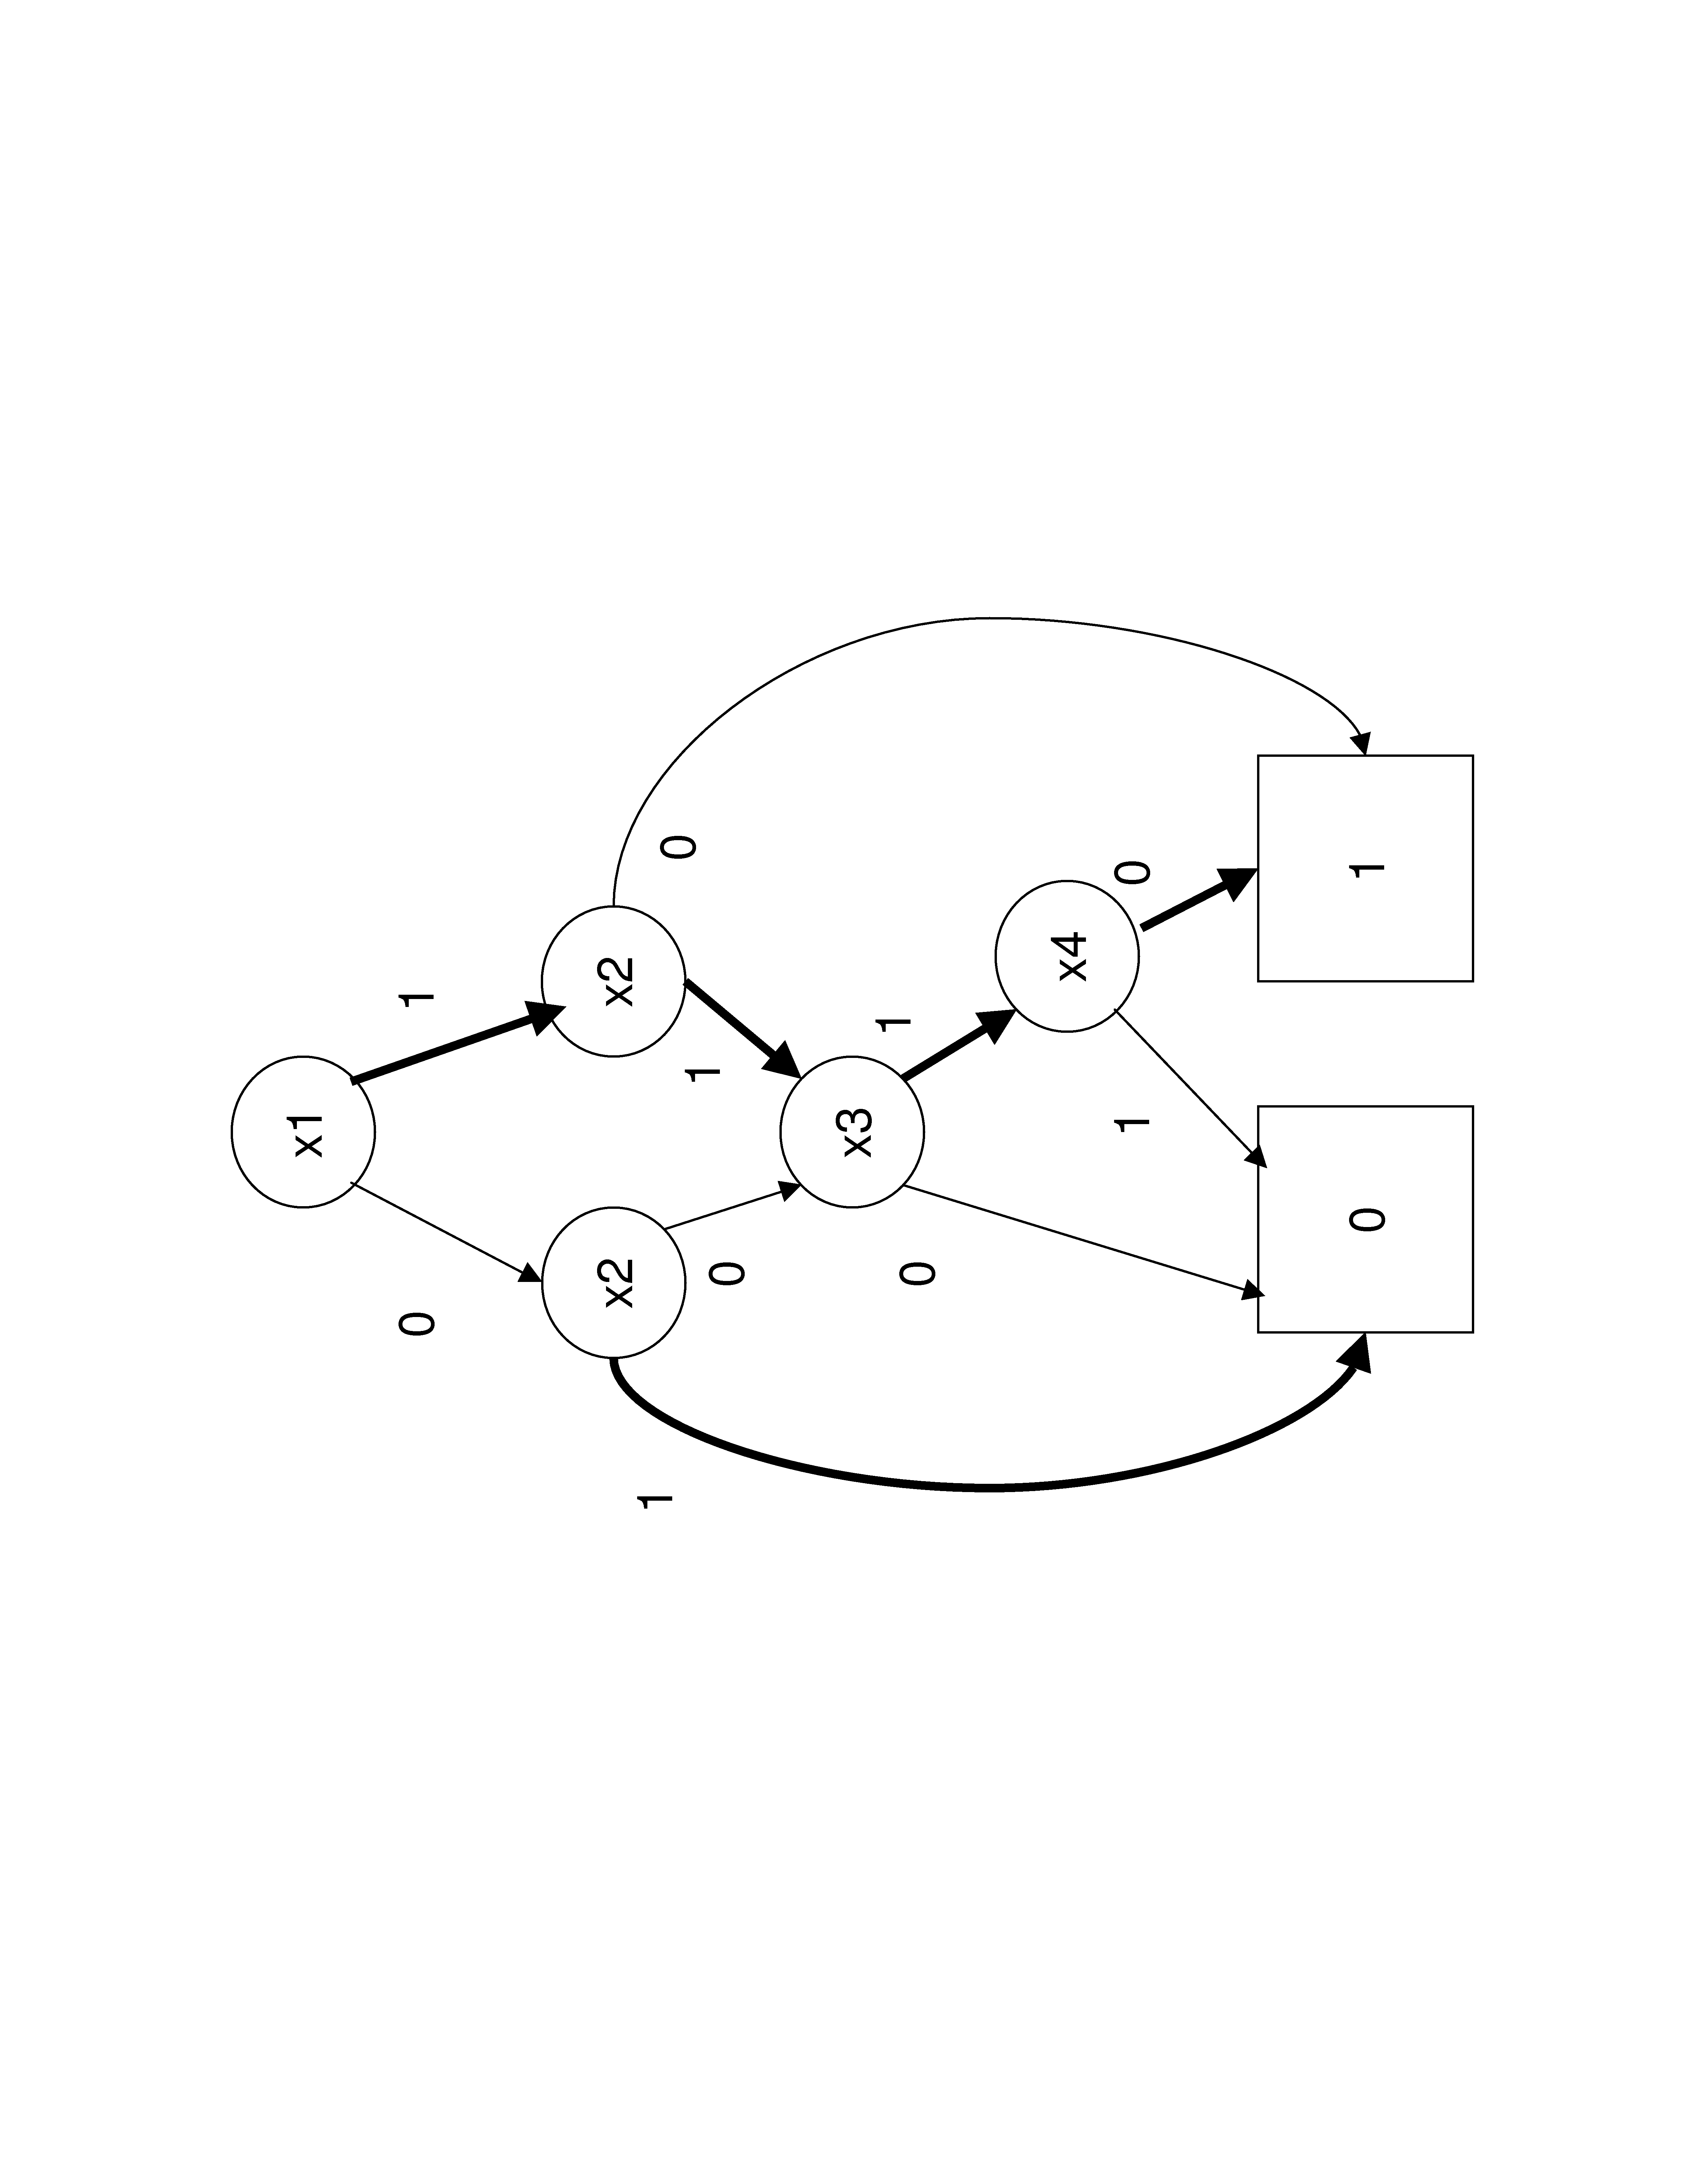
\includegraphics[scale=0.4,angle=270]{chapters/obdd1} 
\par\end{centering}

\caption{\label{fig:OBDD-example}OBDD for two-bit millionaires' problem}

\end{figure}


In \cite{kruger06}, we presented an SFE protocol that directly uses
an OBDD representation of the function $f$ to be jointly computed.
The advantage of using an OBDD representation over the Boolean gate-representation
is that OBDDs are more succinct for certain classes of functions than
the Boolean gate representation, including most linear functions.
For example, the OBDD representation is more efficient than the Boolean
gate representation for 8-bit AND, 8-bit addition, and the millionaires'
and billionaires' problems \cite{Yao86} OBDDs are not a universal
solution, however, for other functions, such as multiplication, the
OBDD can be far worse than the Boolean gate representation, due to
exponential node explosion \cite{Bryant:BDD}. For the classes of
functions in which the OBDD representation is efficient, our thesis
\cite{kruger06} shows that the protocol described next can perform
2 to 4 times better than the classical Yao protocol.

The protocol is loosely designed in a similar fashion as Yao's protocol
\cite{Yao86}. We present two variations of the protocol. An overview
of the 3 main steps of the protocols are shown in figure \ref{fig:OBDD-overview},
using the example millionaires' problem pictured above. In the first
step, Alice sends to Bob the encrypted OBDD. The next step is Bob
acquiring a subset of the encryption keys from Alice using $OT_{2}^{1}$.
In the final step, Bob uses the obtained keys to decrypt a single
path through the OBDD yielding the result of the computation. % A formal description follows. 


%
\begin{figure}
\begin{centering}
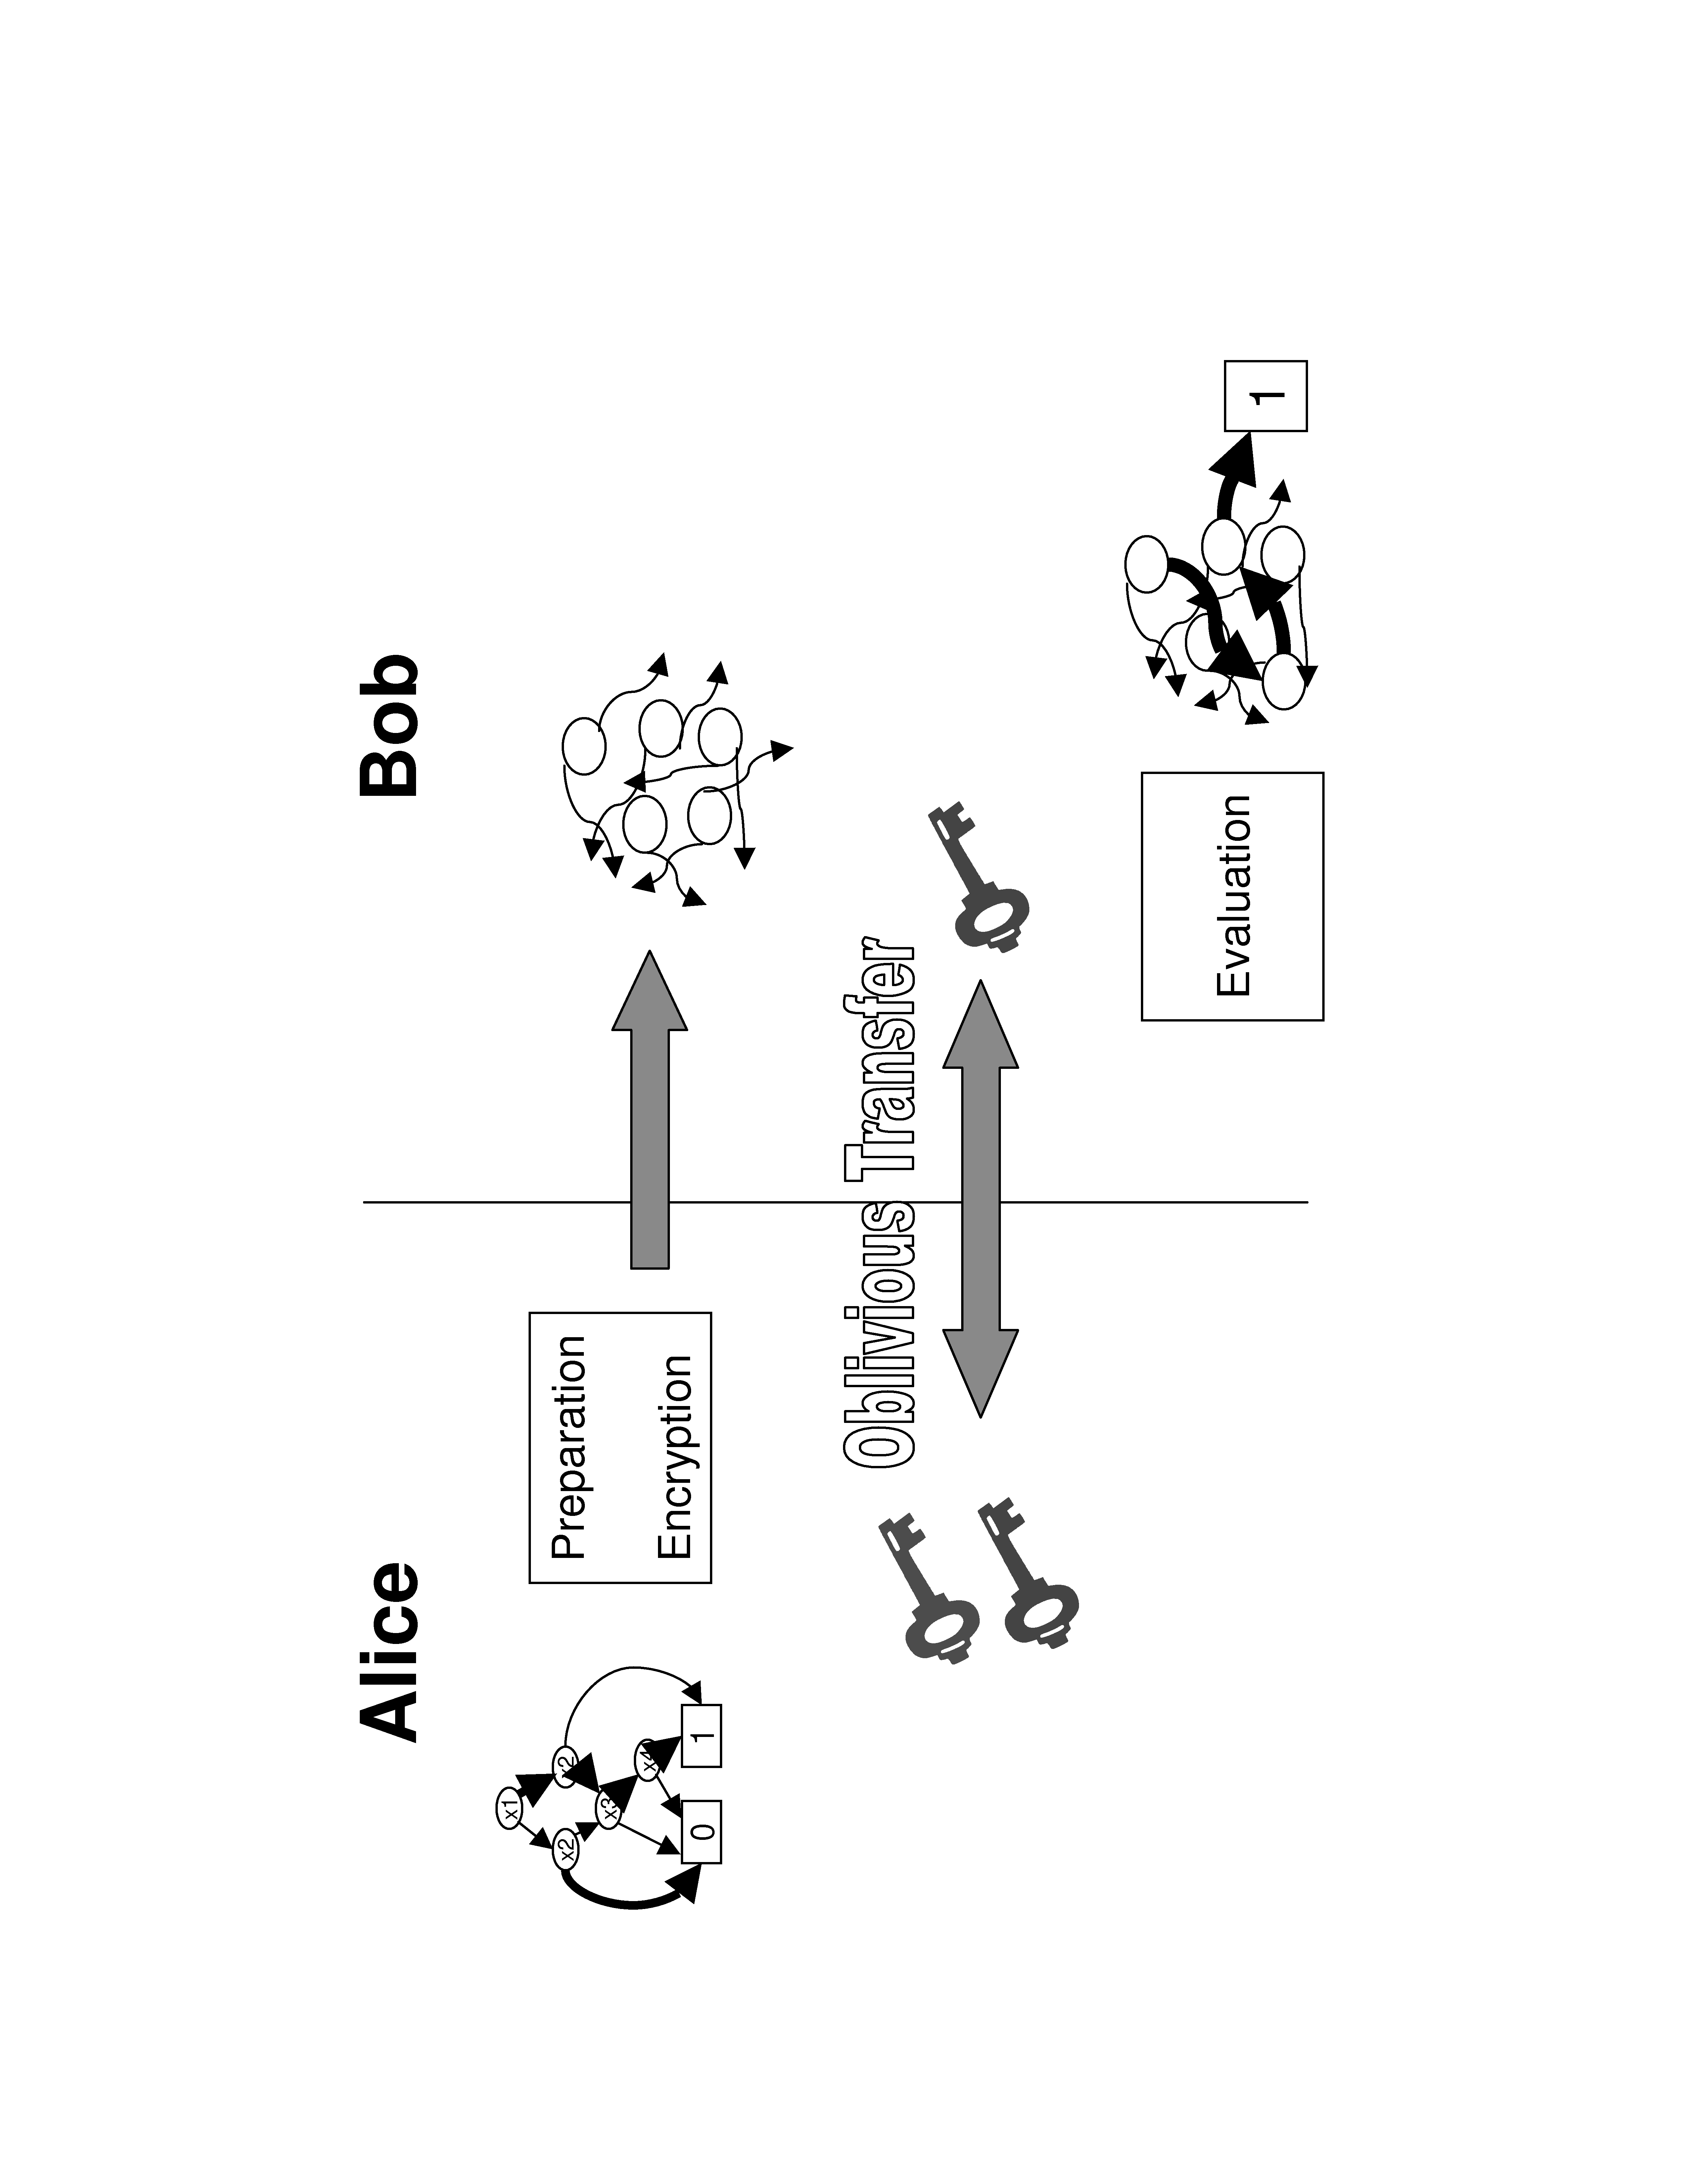
\includegraphics[scale=0.4,angle=270]{chapters/obdd_proto_overview} 
\par\end{centering}

\caption{\label{fig:OBDD-overview}OBDD secure evaluation protocol}

\end{figure}


%\begin{flushleft}
Assume that both parties' inputs include the $OBDD(f)$ for the Boolean
function $f(x_{1},x_{2},\cdots,x_{n})$ with the ordering $x_{1}<x_{2}<\cdots<x_{n}$.
Furthermore, Alice holds the inputs $(i_{1},\ldots,i_{k})$ corresponding
to the first $k$ variables $x_{1},\ldots,x_{k}$, and Bob has the
inputs $(i_{k+1},\ldots,i_{n})$.
\par\end{flushleft}
\begin{enumerate}
\item Alice performs the following steps: 

\begin{enumerate}
\item She traverses the $OBDD(f)$ using her input $(i_{1},\cdots,i_{k})$,
which results in a node $v_{init}$ at level $k$.
\item She uniformly and independently at random creates $(n-k)$ pairs of
secrets $(s_{1}^{0},s_{1}^{1}),\cdots,(s_{n-k}^{0},s_{n-k}^{1})$.
In addition, for each node $v$ in the $OBDD(f)$ whose level is between
$k$ and $n-1$, Alice also creates a secret $s_{v}$.
\item She assigns a uniformly random label to each node whose level is between
$k$ and $n$. We refer to the randomly assigned label of node $v$
using the notation $label(v)$.
\item Next, Alice augments $OBDD(f)$ with some number of dummy nodes (to
ensure that Bob always traverses $n-k$ nodes in his phase of the
protocol).
\item Alice garbles all nodes whose level is between $k$ and $n-1$ in
the following manner. Let $v$ be a node in $OBDD(f)$ such $k\leq{\it level}(v)\leq n-1$
and define ${\it level}(v)=\ell$. The encryption of node $v$, denoted
by $E^{(v)}$, is a label and a randomly ordered ciphertext pair \[
\left(label(v)\,\,,\,\, E_{s_{v}\oplus s_{\ell-k+1}^{0}}(label(low(v))\,\|\, s_{{\it low}(v)})\,\,\,,\,\,\, E_{s_{v}\oplus s_{\ell-k+1}^{1}}(label(high(v))\,\|\, s_{{\it high}(v)})\right)\,\,\,,\]
 where the labels are pre-pended to the secret with a separator symbol
and the order of the ciphertexts is determined by a fair coin flip.
Roughly speaking, the secrets corresponding to the $0$-successor
and $1$-successor of node $v$ are encrypted with the secret corresponding
to $v$ and its level.


Note that dummy nodes have the same structure as normal nodes, except
that the ciphertext pair contain encryptions of the same message since
dummy nodes have the same $0$ and $1$-successors. Provided the encryption
scheme is semantically secure, this poses no problem since the keys
are chosen uniformly at random.

Lastly, there are two terminal nodes of the form $(b,label(t_{b}))$
for $b=0$ or $1$. Recall that $OBDD(f)$ has two terminal nodes,
denoted as $0$ and $1$, that are at level $n$.

\item Once Alice is done encrypting, she sends to Bob the encryption of
all nodes whose level is between $k$ and $n$ and the secret $s_{v_{init}}$
corresponding to node $v_{init}$ at level $k$. We called this the
garbled OBDD.
\end{enumerate}
\item Bob performs the following steps: 

\begin{enumerate}
\item He engages in $n-k$ 1-out-of-2 oblivious transfers to obtain the
secrets corresponding to his input. For example, if his input $i_{j}$
is $0$, then he obtains the (level) secret $s_{j-k}^{0}$; otherwise,
he obtains the secret $s_{j-k}^{1}$.
\item Now Bob is ready to start his computation. Suppose $i_{k+1}=0$. With
$s_{1}^{0}$ and $s_{v_{init}}$, he decrypts both ciphertexts in
$E^{(v_{init})}$ and decides which gives the correct result by using
the verifiable range property of the encryption scheme. Bob now has
both $s_{{\it low}(v)}$ (the secret corresponding to the $0$-successor
of $v_{init}$) and $label(low(v))$ (which tells Bob which encrypted
node is used to evaluate his next input). Continuing this way, Bob
eventually obtains a label corresponding to one of the terminal nodes,
which determines the result of the OBDD on the shared inputs. Bob
sends this result to Alice. 
\end{enumerate}
\end{enumerate}




We then define an optimized variation which is identical to the protocol
just described, except that Alice first reduces the number of nodes
to be sent to Bob using an operation called \emph{restriction}, which
is a partial evaluation applied to OBDDs. Restriction is defined as
follows.

Given an $n$ variable Boolean function $f(x_{1},x_{2},\cdots,x_{n})$
and a Boolean value $b$, the restriction $f\mid_{x_{i}\leftarrow b}$
is a Boolean function of $n-1$ variables $x_{1},\cdots,x_{i-1},x_{i+1},\cdots,x_{n}$.
$f\mid_{x_{i}\leftarrow b}(x_{1},\cdots,x_{i-1},x_{i+1},\cdots,x_{n})$
is equal to $f(x_{1},\cdots,x_{i-1},b,x_{i+1},\cdots,x_{n})$. Essentially,
$f\mid_{x_{i}\leftarrow b}$ is the function obtained by substituting
the value $b$ for the variable $x_{i}$ in the function $f$. The
restriction operation can be performed over multiple variables by
restricting each variable independently, e.g., $f\mid_{x_{i}\leftarrow b,x_{j}\leftarrow b'}=(f\mid_{x_{i}\leftarrow b})\mid_{x_{j}\leftarrow b'}$.
The order in which the variables are restricted is unimportant.

\begin{flushleft}
For protocol 2, both parties' inputs include the $OBDD(f)$ for the
Boolean function $f(x_{1},x_{2},\cdots,x_{n})$ with the ordering
$x_{1}<x_{2}<\cdots<x_{n}$. Furthermore, Alice holds the inputs for
the variables in the set $X_{A}$ and Bob holds the inputs for the
variables in the set $X_{B}\;=\;\{x_{1},\cdots,x_{n}\}-X_{A}$. 
\par\end{flushleft}
\begin{enumerate}
\item Alice performs the following steps:

\begin{enumerate}
\item Alice computes the OBDD ${\cal O}_{A}$ as the restriction of her
inputs on the function $f\mid_{X_{A}}$. 
\item Alice encrypts the $O_{A}$ and sends it to Bob. This step is exactly
the same as in for Protocol 1. Alice also sends the secret corresponding
to the root of the OBDD ${\cal O}_{A}$. 
\end{enumerate}
\item The computation for Bob is exactly the same as that for Protocol 1. 
\end{enumerate}
The results of this work demonstrate that OBDDs showed improved performance
with secure evaluation of certain functions, as will be discussed
in chapter \ref{chapter:obdd}.

%\begin{comment}
\section{Problem Specific: Protocol Optimization of Evaluating Hash Functions
for Password Authentication}

In chapter \ref{chapter:pw}, based on our paper Secure Password Authentication
Using SFE \cite{Kruger10}, we use some properties of the problem
of authentication to transform the semi-honest protocol into an efficient
protocol that is secure in the malicious model. This work presents
a new solution to the {}``Secure Password and Key Authentication''
(SPAKA) problem, which is the design of protocols to mutually authenticate
a client to a server using 
\begin{enumerate}
\item The client's knowledge of the password X, and 
\item The servers's knowledge of a one-way hash function h(X). 
\end{enumerate}
The protocol must not leak any additional information or allow access
if one of the parties is an inposter and does not know their expected
credential. Our solution provides a property, unique among SPAKA protocols,
that it can work with arbitrary and legacy hash functions used in
commodity operating systems today. This protocol takes advantage of
specific properties of the authentication problem and takes {}``shortcuts''
to achieve efficiency. Although these shortcuts would not be secure
in a general SFE setting, we prove that these shortcuts are in fact
secure in the context of the authentication protocol presented. This
allows us to design a protocol in which a malicious adversary is thwarted
with probability $1-2^{-l}$ where $l$ is a security parameter representing
the number of semi-honest circuits. We show that on modern multicore
processors, the authentication can be performed in a matter of seconds,
which we believe is practical for interactive use between servers
and authenticating users.
%\end{comment}

\section{Class of Algorithm Specific: Protocol Optimization of Dynamic Programming}

In this work, presented in detail in chapter \ref{chapter:genomics},
we considered a design \emph{methodology} for creating secure protocols
based on typical dynamic programming algorithms. Unlike the OBDD protocol
discussed in the previous section, this is not an automatic tool for
generating secure protocols, but rather a set of concepts that are
applicable to designing secure protocols for evaluating dynamic programming
algorithms. We illustrate these ideas with several example protocols
for computing the edit distance problem, which is the minimum number
of character insertions, deletions, and substitutions needed to change
string $x$ to string $y$.

Let ${\cal P}(x,y)$ be a problem with two inputs $x$ and $y$. Typically,
a dynamic-programming algorithm ${\cal A}_{{\cal P}}$ for problem
${\cal P}$ has the following components: 
\begin{itemize}
\item A set $S$ of sub-problems and a dependency relation $R\subseteq S\times S$
between the sub-problems. Intuitively, $(s,s')\in R$ means that the
sub-problem $s'$ depends on the sub-problem $s$. If there is a dependency
between $s$ and $s'$, we write it as $s\rightarrow s'$. In the
case of the problem of computing edit-distance between two strings
$\alpha$ and $\beta$ of length $n$ and $m$, the set of sub-problems
is $[0,\cdots,n]\times[0,\cdots,m]$. For all sub-problems $(i,j)$
such that $i\not=0$ and $j\not=0$, we have the following dependencies:
$(i-1,j)\rightarrow(i,j)$, $(i,j-1)\rightarrow(i,j)$, and $(i-1,j-1)\rightarrow(i,j)$.
The \textit{base sub-problems} are $s\in S$ such that they have no
dependencies. For the edit-distance problem, the base sub-problems
are: \[
\begin{array}{l}
\{(i,0)\;\mid\;0\leq i\leq n\}\\
\{(0,j)\;\mid\;0\leq j\leq m\}\end{array}\]
 We also assume that there is a unique root sub-problem ${\it root}\in S$
such that there does not exist a sub-problem that depends on ${\it root}$.
For the edit-distance problem the unique root sub-problem is $(n,m)$. 
\item Each sub-problem $s$ is assigned a value ${\it val}(s)$. The goal
is to compute ${\it val}({\it root})$. The function ${\it val}$
from $S$ to $\Re$ assigns values to sub-problems, such that it satisfies
the following properties:

\begin{itemize}
\item For all the base sub-problems $s\in S$, ${\it val}(s)$ is defined. 
\item Let $s\in S$ be a non-base sub-problem. Define ${\it pred}(s)$ as
all the predecessors of $s$, i.e. the set ${\it pred}(s)$ is defined
as $\{s'\;\mid\; s'\rightarrow s\}$. Assume that ${\it pred}(s)$
is equal to $\{s_{1},\cdots,s_{k}\}$. There is a recursive function
$f$ defining ${\it val}(s)$ in terms of ${\it val}(s_{1}),{\it val}(s_{2}),\cdots,{\it val}(s_{k})$,
$s(x)$, and $s(y)$, where $s(x)$ and $s(y)$ are parts of the input
$x$ and $y$ that are relevant to the sub-problem $s$. In case of
the edit-distance problem ${\it val}((i,j))$ is equal to $D(i,j)$. 
\end{itemize}
\end{itemize}
We implemented three variations of the protocol in \cite{kruger07},
and showed that the techniques produce efficient ways to compute the
edit distance of two strings. For example, the protocol is able to
compute the edit distance of two strings of length $200$ (which has
$200^{2}=40000$ sub-computations), in under 10 minutes. Our most
efficient protocol computes elements of the dynamic programming matrix
in large blocks during each round of the computation. We experimentally
determined than a block size of $(20,20)$ yielded an optimum trade-off
between a decreased number of rounds, and larger block circuits. Using
a $(20,20)$ circuit allows $20^{2}=400$ elements of the matrix to
be evaluated during each round of the protocol, which allows the overall
$(200,200)$ problem to be evaluated in $100$ rounds. In comparison,
using the generic techniques to compile the edit distance algorithms
into a secure circuit produced circuits which were to too large for
evaluation beyond problems of size $(25,25)$.


\section{Algorithm Specific: Protocol Optimization of K-Means Clustering}

The $k$-means algorithm is a common clustering technique in data
mining. Suppose that we are given $n$ samples $x_{1},\cdots,x_{n}$,
where each sample is a $m$-dimensional vector of real numbers. The
problem is to assign the samples to $c$ clusters in such a manner
that similar points are grouped together. Similarity is defined using
a distance metric. The standard clustering algorithm maintains $c$
means $\mu_{1},\cdots,\mu_{c}$. Initially, assume that the means
are assigned arbitrary values. A sample $x_{i}$ is deemed to be in
the cluster $j$ if it is closest to the mean $\mu_{j}$, where mean
of a cluster $\{x'_{1},\cdots,x'_{r}\}$ is $\frac{x'_{1}+\cdots,x'_{r}}{r}$.
In a Euclidean space, the distance between two $m$-dimensional vectors
$x$ and $y$ is $\sum_{j=1}^{m}(x[j]-y[j])^{2}$, where $x[j]$ is
the $j$-th element of the vector $x$. Other distance metrics~\cite[Chapter 10]{pattern-classification},
such as scatter metrics, can be used instead of the distance metric
mentioned above. Each iteration of the $k$-means algorithms recomputes
the means and reclassifies the samples. The algorithm terminates when
it detects no change in the means. See \ref{fig:clusters} for an
illustration.

%
\begin{figure}
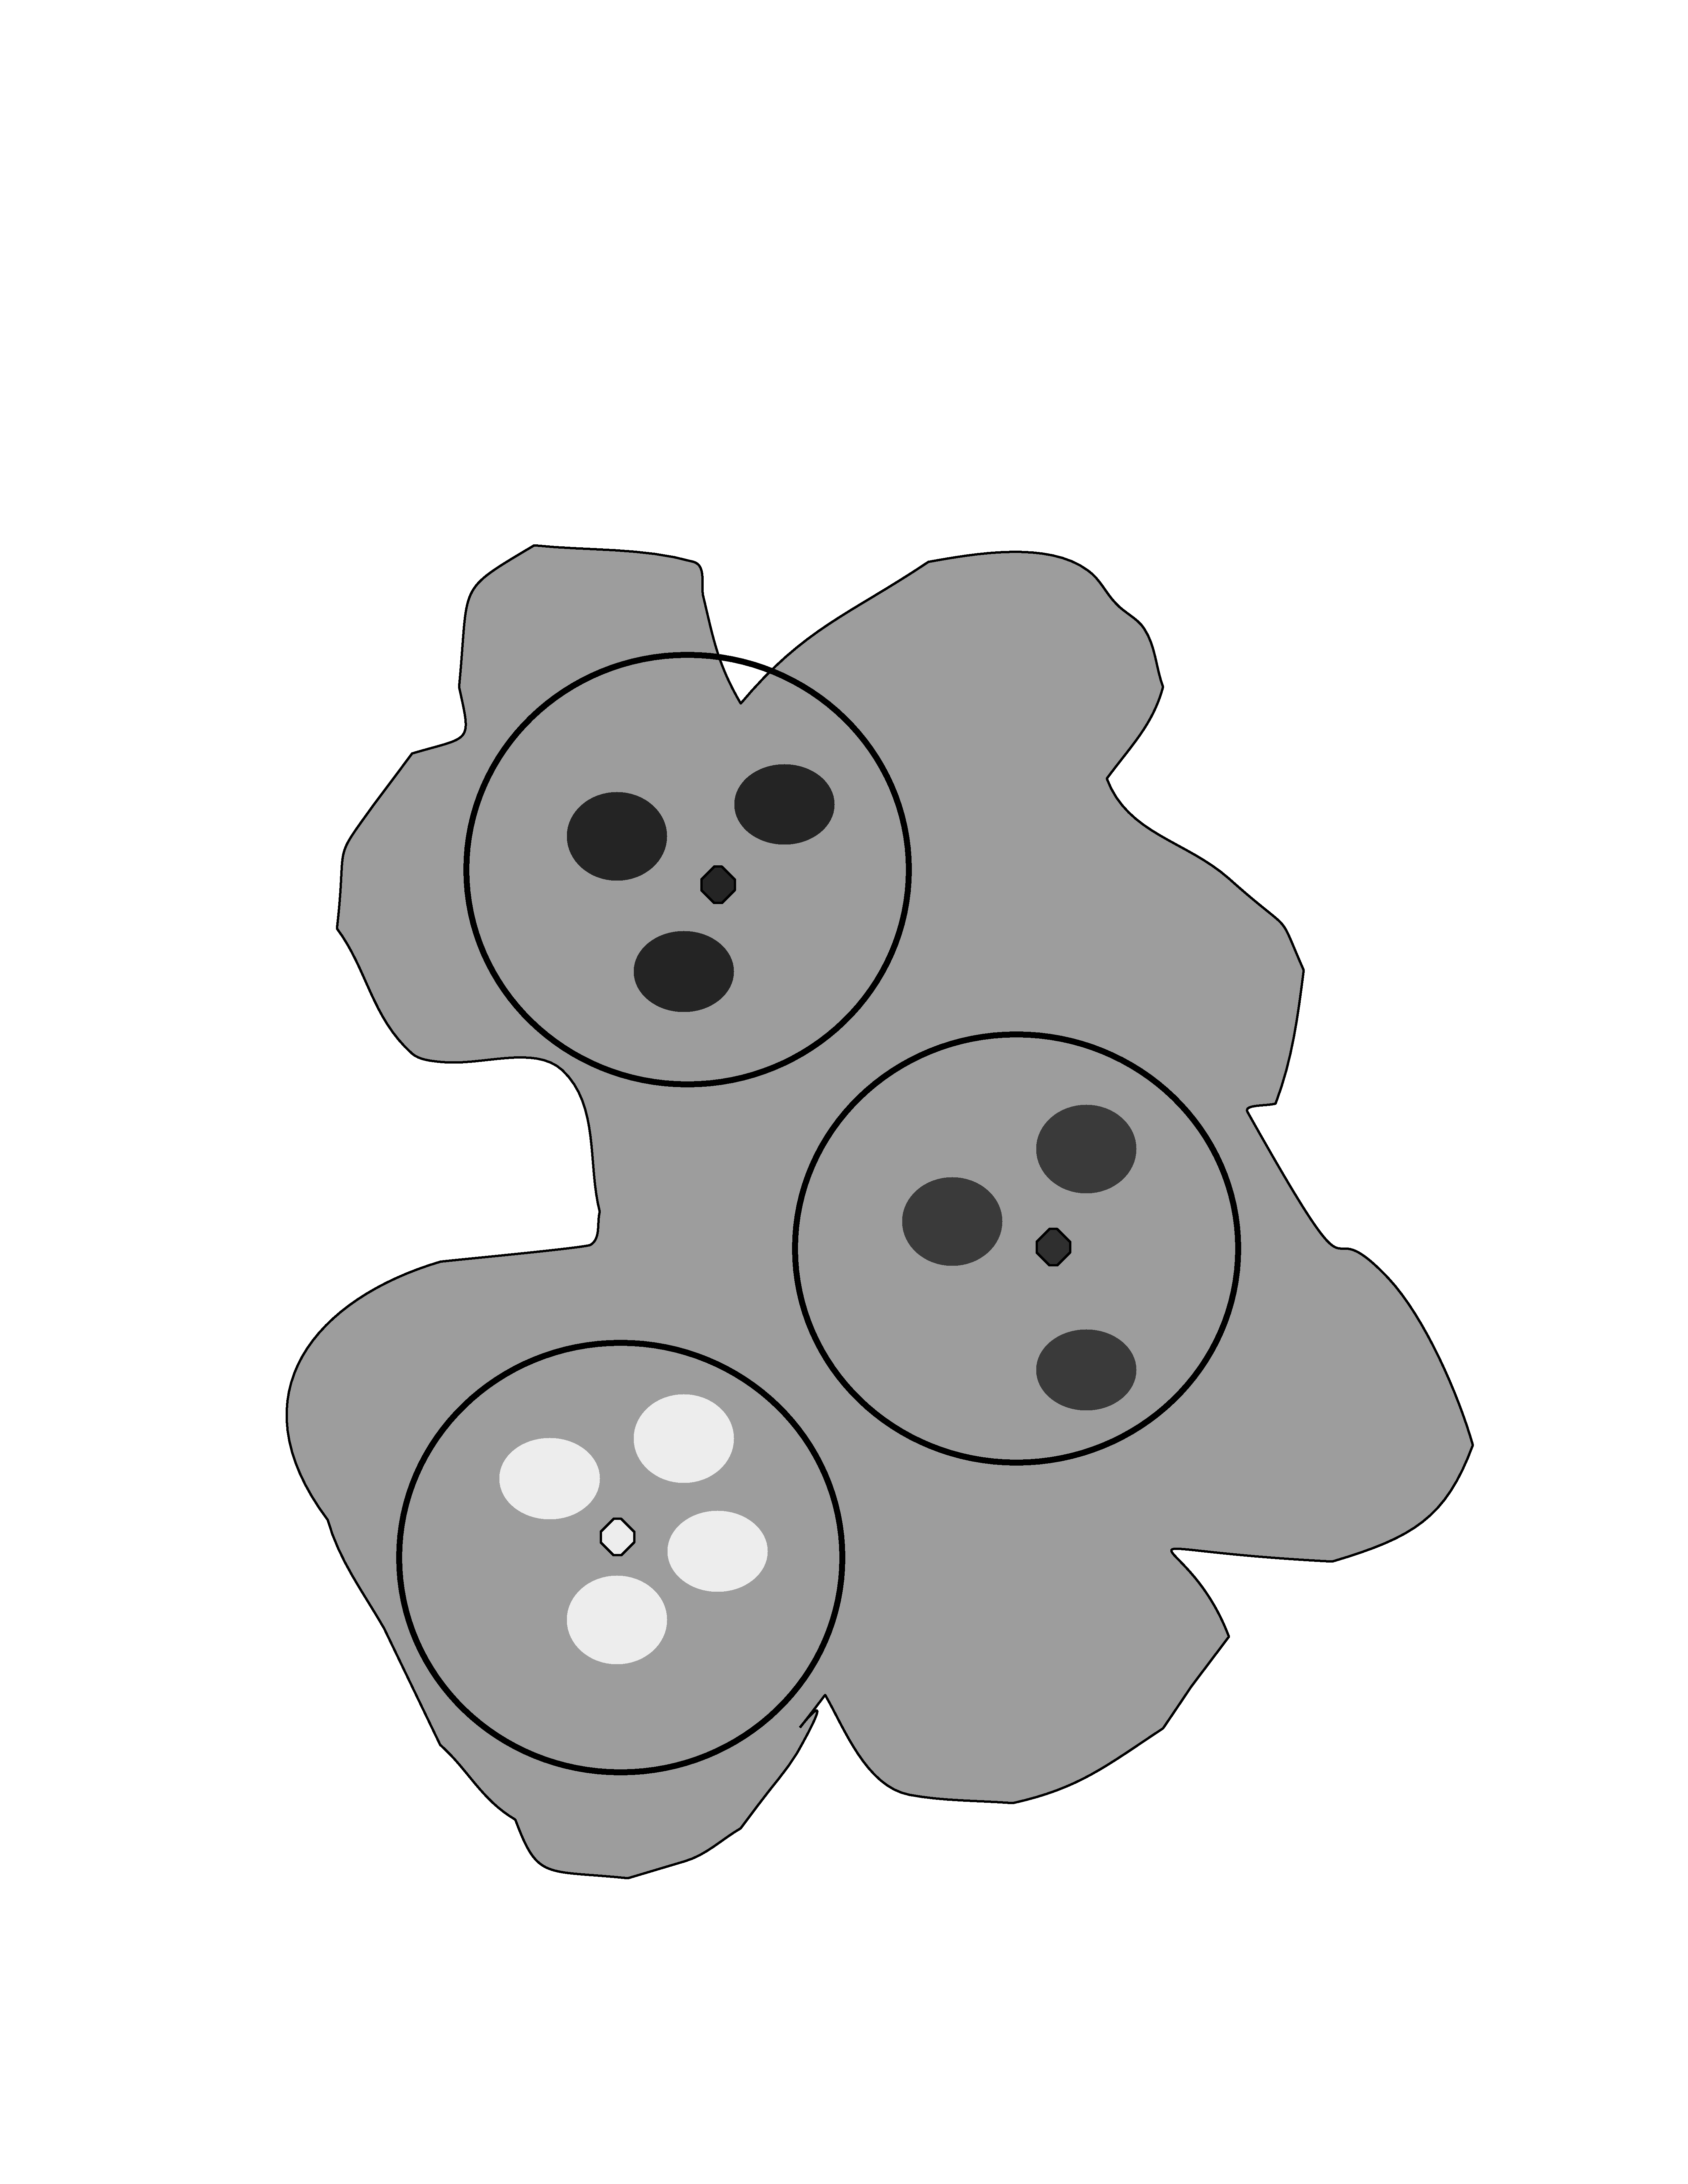
\includegraphics[scale=0.3,angle=270]{chapters/clusters}

\caption{\label{fig:clusters}Thirteen data points after clustering. The small
dots are cluster means.}

\end{figure}


We implement protocols to securely evaluate this algorithm in chapter
\ref{chapter:kmeans} based on our paper \cite{kruger05}, and showed
that a protocol based on homomorphic encryption was able to classify
partitioned data sets with tens of thousands of data points in under
two minutes, which is about 15 times slower than the protocol implemented
without privacy protection, and over 100 times faster than the same
protocol built with Yao circuits.


\section{Other Optimizations}

\label{sub:Other-Optimizations}

In the usual formulation of secure function evaluation, there are
designated outputs for each party, and it is required that no extra
information is learned by any party. This definition could be expanded
to assign non-output values the labels {}``sensitive'' and {}``non-sensitive'',
where the protocol is considered secure if no sensitive information
is leaked. %Since the overhead of privacy protection is substantial,
%I propose to research the of design secure protocols that use this
%relaxation of the problem definition to improve efficiency. 


In section \ref{sub:Primitives}, I presented many basic cryptographic
primitives that are used in SFE. Improving the state of the art of
any one of those primitives would automatically benefit all SFE protocols
that make use of that primitive. Based on my experience with real
implementations of SFE protocols, the oblivious transfer steps tend
to be very expensive in terms of space and communication. Common oblivious
transfer protocols are based on discrete logarithms, but other trapdoor
functions may be used as well. %One thing I propose to try is implementing
%Naor-Pinkas \cite{Noar-Pinkas:2001} using more compact representations,
%for example, with elliptic curve groups. I have recently developed
A new $OT_{2}^{1}$ protocol is presented in chapter \ref{sec:OT-SquareRoots}.
and its security and performance are compared with the Naor-Pinkas
protocol. %In particular, I conjecture that this protocol
%may require less communication overhead than other OT protocols.


%
\begin{comment}

\chapter{An Efficient Protocol Design Framework}

\label{sub:An-Efficient-Framework}

Even with all these optimizations, protocols still must be hand-coded.
Each protocol I have implemented has required brand new code to be
written, with only some common cryptographic primitives being shared
between implementations. In this case, I define the term protocol
to mean a structured sequence of communications between parties which
enables the computation to performed. Fairplay \cite{Fairplay} suggested
the idea of having a common framework for protocol design, but because
Fairplay is a straightforward implementation of Yao's garbled circuit
method \cite{Yao86}, it suffers from poor performance. Fairplay's
contribution is to create a compiler for expressing algorithms functionally,
and compiling them into a circuit representation suitable for secure
evaluation. In this sense, it functions as a simple CAD design tool.

I propose to take this concept much further, and create an \emph{optimizing}
protocol compiler, aggregating the techniques discussed here, and
creating a tool to greatly simplify the creation of efficient secure
protocols for SFE. The compiler will include the following components: 
\begin{itemize}
\item Convenient programming language for expressing secure computations

\begin{itemize}
\item Language will include support as language primitives for common SFE
and cryptographic techniques, such as homomorphic encryption 
\item Language will support metadata for designating inputs and outputs
from specific parties, and for classifying the required privacy of
intermediate computations 
\end{itemize}
\item Compiler which translates this language into an abstract securely
evaluable {}``machine code'', which consists of securely evaluable
representations of the program. 
\item An automated optimizer. The optimizer will automatically try different
representations of the functions, including OBDDs, Boolean circuits,
and other ideas from my research, and search for the most efficient
representation as possible. 
\item Manual optimization tools, making it convenient to apply and design
techniques that I have researched. This includes a toolkit of cryptographic
protocols, such as oblivious transfer, which can be used in a black
box way. 
\item An embeddable protocol evaluator library, which will allow ordinary
application to make straightforward use of secure function evaluation. 
\end{itemize}
The security of protocols produced by the compiler is based on the
security of each individual component of the protocol. For example,
when choosing optimal circuit representations, the compiler will choose
among several possible representations, each of which has a corresponding
secure evaluation protocol. In cases where a computation is broken
into multiple sub-protocols, I will prove that composition of these
sub-protocols maintains the overall security of the protocol.

\bibliographystyle{plain} \bibliographystyle{plain}
\bibliography{somesh}

\end{comment}
{} 



\chapter{Oblivious Transfer with Modular Square Roots}\label{sec:OT-SquareRoots}
\label{chapter:otquad}

A new $OT_{2}^{1}$ protocol is presented, using the square root function
in modular multiplicative groups as a trapdoor function. Here, I present
a informal sketch of correctness, security, and efficiency. I propose
to complete the proofs and perform a thorough experimental evaluation
of its performance with respect to other oblivious transfer protocols.


\section{Protocol}
\begin{enumerate}
\item The sender chooses large random prime numbers $p$ and $q$ such that
$p\equiv q\equiv3\;(\mbox{mod }4)$ and calculates $n=pq$. $n$ is
sent to the chooser. This is a one time setup step that need not be
repeated for subsequent uses of the protocol.
\item The chooser uniformly chooses a random value $x\in S\subset Z_{n}^{*}$
where $S=\{z\in Z_{n}^{*}:$~$z\le\frac{n-1}{2}\mbox{ and }$ $\left(\frac{z}{n}\right)=-1$
if $s=1$ otherwise $\left(\frac{z}{n}\right)=+1\}$. The chooser
computes $y\equiv x^{2}(\mbox{mod }n)$ and sends $y$ to the sender.
$\left(\frac{x}{n}\right)$ denotes the Jacobi symbol of $x$ and
$n$.
\item The sender calculates the square roots $a^{2}\equiv b^{2}\equiv y\;(mod\, n)$
such that $\left(\frac{a}{n}\right)=-1$ and $\left(\frac{b}{n}\right)=+1$
and $a,b\le\frac{n-1}{2}$
\item The sender encrypts $E_{a}(m_{1})$ and $E_{b}(m_{2})$ and sends
them to the chooser.
\item The chooser computes $D_{x}(E_{x}(m_{s}))$ to decrypt the output.
\end{enumerate}

\section{Correctness}

$\left(\frac{x}{n}\right)=-1$ for half the elements $x\in Z_{n}^{*}$
. $\left(\frac{x}{n}\right)=+1$ for the other half. Thus the chooser
can always successfully perform step 2.

If $a^{2}\equiv b^{2}\;(mod\; n)$ and $a\neq\pm b\;(mod\; n)$ then
$\left(\frac{a}{n}\right)=-\left(\frac{b}{n}\right)$.%
\footnote{This follows when $p\equiv q\equiv3\ (\mbox{mod 4})$ from the properties
of the Jacobi symbol and the Chinese Remainder Theorem.%
} Furthermore, the set $\{a,b,n-a,n-b\}$is the complete set of square
roots of $y$. If $a>\frac{n-1}{2}$ then $a$ and $n-a$ can be swapped,
and similarly for $b$. Thus, the sender can always successfully complete
step 3. It is guaranteed that either $a=x$ or $b=x$ so the chooser
will successfully learn $m_{s}$ as intended.


\section{Security}

Finding all square roots of any quadratic residue in $Z_{n}^{*}$
can be reduced to factoring $n$. This is because given two principal
square roots $a^{2}\equiv b^{2}$, $a\neq-b$, then $(a-b)(a+b)\equiv0$
so $(a-b)(a+b)=kpq$ Under the standard complexity assumption that
factoring $n$ is infeasable, then the chooser can not efficiently
learn the other square root of $x^{2}$, which is the encryption key
of $E(m_{3-s})$ and the sender's privacy is preserved. 

The chooser's privacy is preserved because the sender does not know
whether the chooser calculated $y=a^{2}$ or $y=b^{2}$. From the
sender's perspective, the chooser has chosen $x$ from a uniform random
distribution $1\le x\le\frac{n-1}{2}$, so there is no information
that can be gained. The chooser therefore enjoys unconditional security
even without making assumptions about the senders computation power.


\section{Efficiency}

In the setup phase, the sender needs to calculate $n=pq$ once and
send the value of $n$ to the chooser. This requires one multiplication
and transmission of $k=\log n$ bits. The same value of $n$ can be
reused for subsequent or batched OTs without loss of security. $k$
must be large enough to prevent efficient factoring of $n$.

From then on, each OT requires the following: 
\begin{enumerate}
\item Computation of Jacobi symbols $\left(\frac{x}{n}\right)$ by the chooser.
If the chooser uses random trials to find an appropriate $x$, then
the expected number of trials is $2$. Computing Jacobi symbols can
be performed in $O(k\log x)\le O(k^{2})$ steps \cite{1996-bach-book}. 
\item There is a potential optimization of step 1. The chooser can pre-compute
a single number $\alpha$ where $\left(\frac{\alpha}{n}\right)=-1$.
From then on, the chooser can choose any random $\beta$ and have
$\left(\frac{\beta^{2}}{n}\right)=+1$ and $\left(\frac{\alpha\beta^{2}}{n}\right)=-1$.
This optimization as presented is insecure, because it breaks statistical
indistinguishability for the chooser~%
\footnote{The optimization will never produce a non-QR with $+1$ Jacobi symbol%
}. However, I speculate that there may exist a variation which avoids
this flaw and thereby reduces the chooser's overall complexity to
$O(k)$.
\item Transmission of a single $k$ bit number from chooser to sender
\item Computation by the sender of square roots of $y$. This can be performed
using a randomized algorithm in expected time $O(k\ \log\, p^{2})\le O(k^{3})$
steps for $p>q$ \cite{1996-bach-book}. 
\item Encryption and transmission by the sender of the two messages. If
the sender does not need to hide the length of the unreceived message,
then this requires no more bandwidth than the actual size of the messages,
which is $O(\log m)$
\item Decryption by the receiver of one of the messages, which is $O(\log m)$.
\end{enumerate}
If the sender and chooser wish to execute the protocol multiple times,
the chooser can simply send a vector $[y_{1},\cdots,y_{j}]$ and the
chooser will respond with a vector of tuples $[(E_{a_{1}}(m_{1_{1}}),(E_{b_{1}}(m_{1_{2}}))\cdots(E_{a_{j}}(m_{j_{1}}),(E_{b_{j}}(m_{j{}_{2}}))]$
where $j$ is the number of messages to be sent obliviously. Each
$x_{i}$ is an independent random variable so the security is equivalent
to the single message case. Thus, unlimited bits can be transferred
with a single network round-trip.


\section{Comparison with Naor-Pinkas\label{sub:Comparison-with-Naor-Pinkas}}

In the Naor-Pinkas protocol \cite{Noar-Pinkas:2001}, the computational
requirement for each party is $O((\log n)(\log\log n))$ for both
parties, where $n$ is the size of a group sufficiently large such
that calculating discrete logarithms is infeasible. The communication
consists of a message of size $\log n$ from sender to chooser, a
message of size $\log n$ from chooser to sender, and two messages
of size $\log m+\log n$ from sender to chooser, where $\log m$ is
the size of the chooser's outputs. The protocol presented here cuts
the final messages to $\log m$, which effectively reduces the bandwidth
with a tradeoff in computation time. My experimentation with running
SFE algorithms using fast modern CPUs indicates that this tradeoff
may be worthwhile. I plan to make empirical measurements with implementations
of the to comparitively measure the actual performance.


\section{Extensions}

It may be possible to extend the construction to cover the more general
$OT_{k}^{1}$. I have not investigated this yet, but one idea is to
let $n=\prod_{i=1}^{k}p_{i}$ where each $p_{i}$ is a large prime
number. In $Z_{n}^{*}$, each quadratic residue will have $2^{k}$
square roots consisting of $2^{k-1}$ pairs $(x,n-x)$

%
\begin{comment}
\bibliographystyle{plain}
\bibliography{crypto,privacy,somesh}

\end{comment}
{}




%
\begin{comment}
\input{newidea.tex}
\end{comment}
{}

%% LyX 1.6.1 created this file.  For more info, see http://www.lyx.org/.
%% Do not edit unless you really know what you are doing.
\documentclass[english]{article}
\usepackage[T1]{fontenc}
\usepackage[latin9]{inputenc}
\usepackage{geometry}
\geometry{verbose,letterpaper,tmargin=1.25in,bmargin=1.25in,lmargin=1.25in,rmargin=1.25in}
\setlength{\parskip}{\medskipamount}
\setlength{\parindent}{0pt}
\usepackage{verbatim}
\usepackage{graphicx}

%%%%%%%%%%%%%%%%%%%%%%%%%%%%%% Textclass specific LaTeX commands.
\newenvironment{lyxcode}
{\par\begin{list}{}{
\setlength{\rightmargin}{\leftmargin}
\setlength{\listparindent}{0pt}% needed for AMS classes
\raggedright
\setlength{\itemsep}{0pt}
\setlength{\parsep}{0pt}
\normalfont\ttfamily}%
 \item[]}
{\end{list}}

%%%%%%%%%%%%%%%%%%%%%%%%%%%%%% User specified LaTeX commands.

\linespread{1.1}

\usepackage{babel}

\begin{document}

\section{Strengthening SSH Password Authentication}

\subsection{Overview}

SSH is the predominant application for interacting with remote
systems. It was designed as an alternative to telnet with the purpose
of addressing the growing need for confidentiality, authentication,
and integrity. It has since evolved into a layered protocol, that can
serve as a secure transport layer over which other protocols can run
for enhanced security. This has increased its popularity to the point
where many of its users simply assume that it provides all of the
security they need.

However, SSH is currently vulnerable to a man in the middle attack
that allows the perpetrator to impersonate either the client or
server, or compromise the client's password. Many assume that this is
not the case because of SSH's host key authentication mechanism, but
there are a number of ways that an attacker can thwart the protection
it provides. For example, any SSH user is certainly familiar with the
following type of message:
\begin{verbatim}
   The authenticity of host 'server (1.2.3.4)' can't be established.
   RSA key fingerprint is 3f:76:22:43:c2:03:b9:71:b0:31:ce:87:37:45:cb:02. 
   Are you sure you want to continue connecting (yes/no)?
\end{verbatim}
In many usage scenarios, it is unreasonable to expect that the client
has verifiable access to the host's RSA key fingerprint before
attempting connection. In these cases, the user is left with a tough
decision; either accept the key's authenticity with no real evidence,
or forgo access to the host's services. This gives an attacker
leverage, and a likely chance at success.

Recent research in related areas has seen the development of a class
of authentication protocols dubbed SPAKA (\textit{Secure Password and
  Key Authentication})~\cite{bellovin92}. SPAKA protocols are designed
to guarantee confidentiality of secrets even against active
adversaries. A recent SPAKA protocol for resisting password compromise
in the event of host compromise~\cite{brainard03} suggests that secure
function evaluation can be applied generally to the problem of
developing SPAKA protocols.

With this in mind as a starting point, we apply SFE to the problem of
developing a SPAKA protocol suitable for authenticating SSH
connections, thus thwarting the MITM attack described earlier. Using
the client's password on the host as a shared secret, we observe that
the authenticity of the host (and the client) can be verified by
securely computing a variant of the millionaire problem. Specifically,
we provide the two parties with a way of determining whether the other
has access to the shared secret, without potentially revealing the
secret to a potential adversary.

In the following sections, we outline the relevant aspects of the SSH
protocol (Section 1.2), detail the nature of the man in the middle
attack on SSH's authentication mechanism (Section 1.3), present our
proposed solution in further detail (Section 1.4), describe our
implementation (Section 2), and talk about related work (Section 3).


\subsection{SSH Protocol Overview}

The SSH protocol is defined in terms of layers, much like the OSI
networking stack. Each layer is defined in terms of messages from the
underlying layer. The lowest level is a packet-based transport
protocol that is layered on top of TCP. All SSH messages of the higher
layers are sent as packets. This packet protocol is known as the SSH
transport layer protocol and is defined in \cite{rfc4253}.  Figure
\ref{fig:ssh-overview} shows the hierarchy of the ssh protocol layers
discussed here. The SSH transport layer also handles the server key
authentication, encryption, and integrity of a session.

%
\begin{figure}[t]
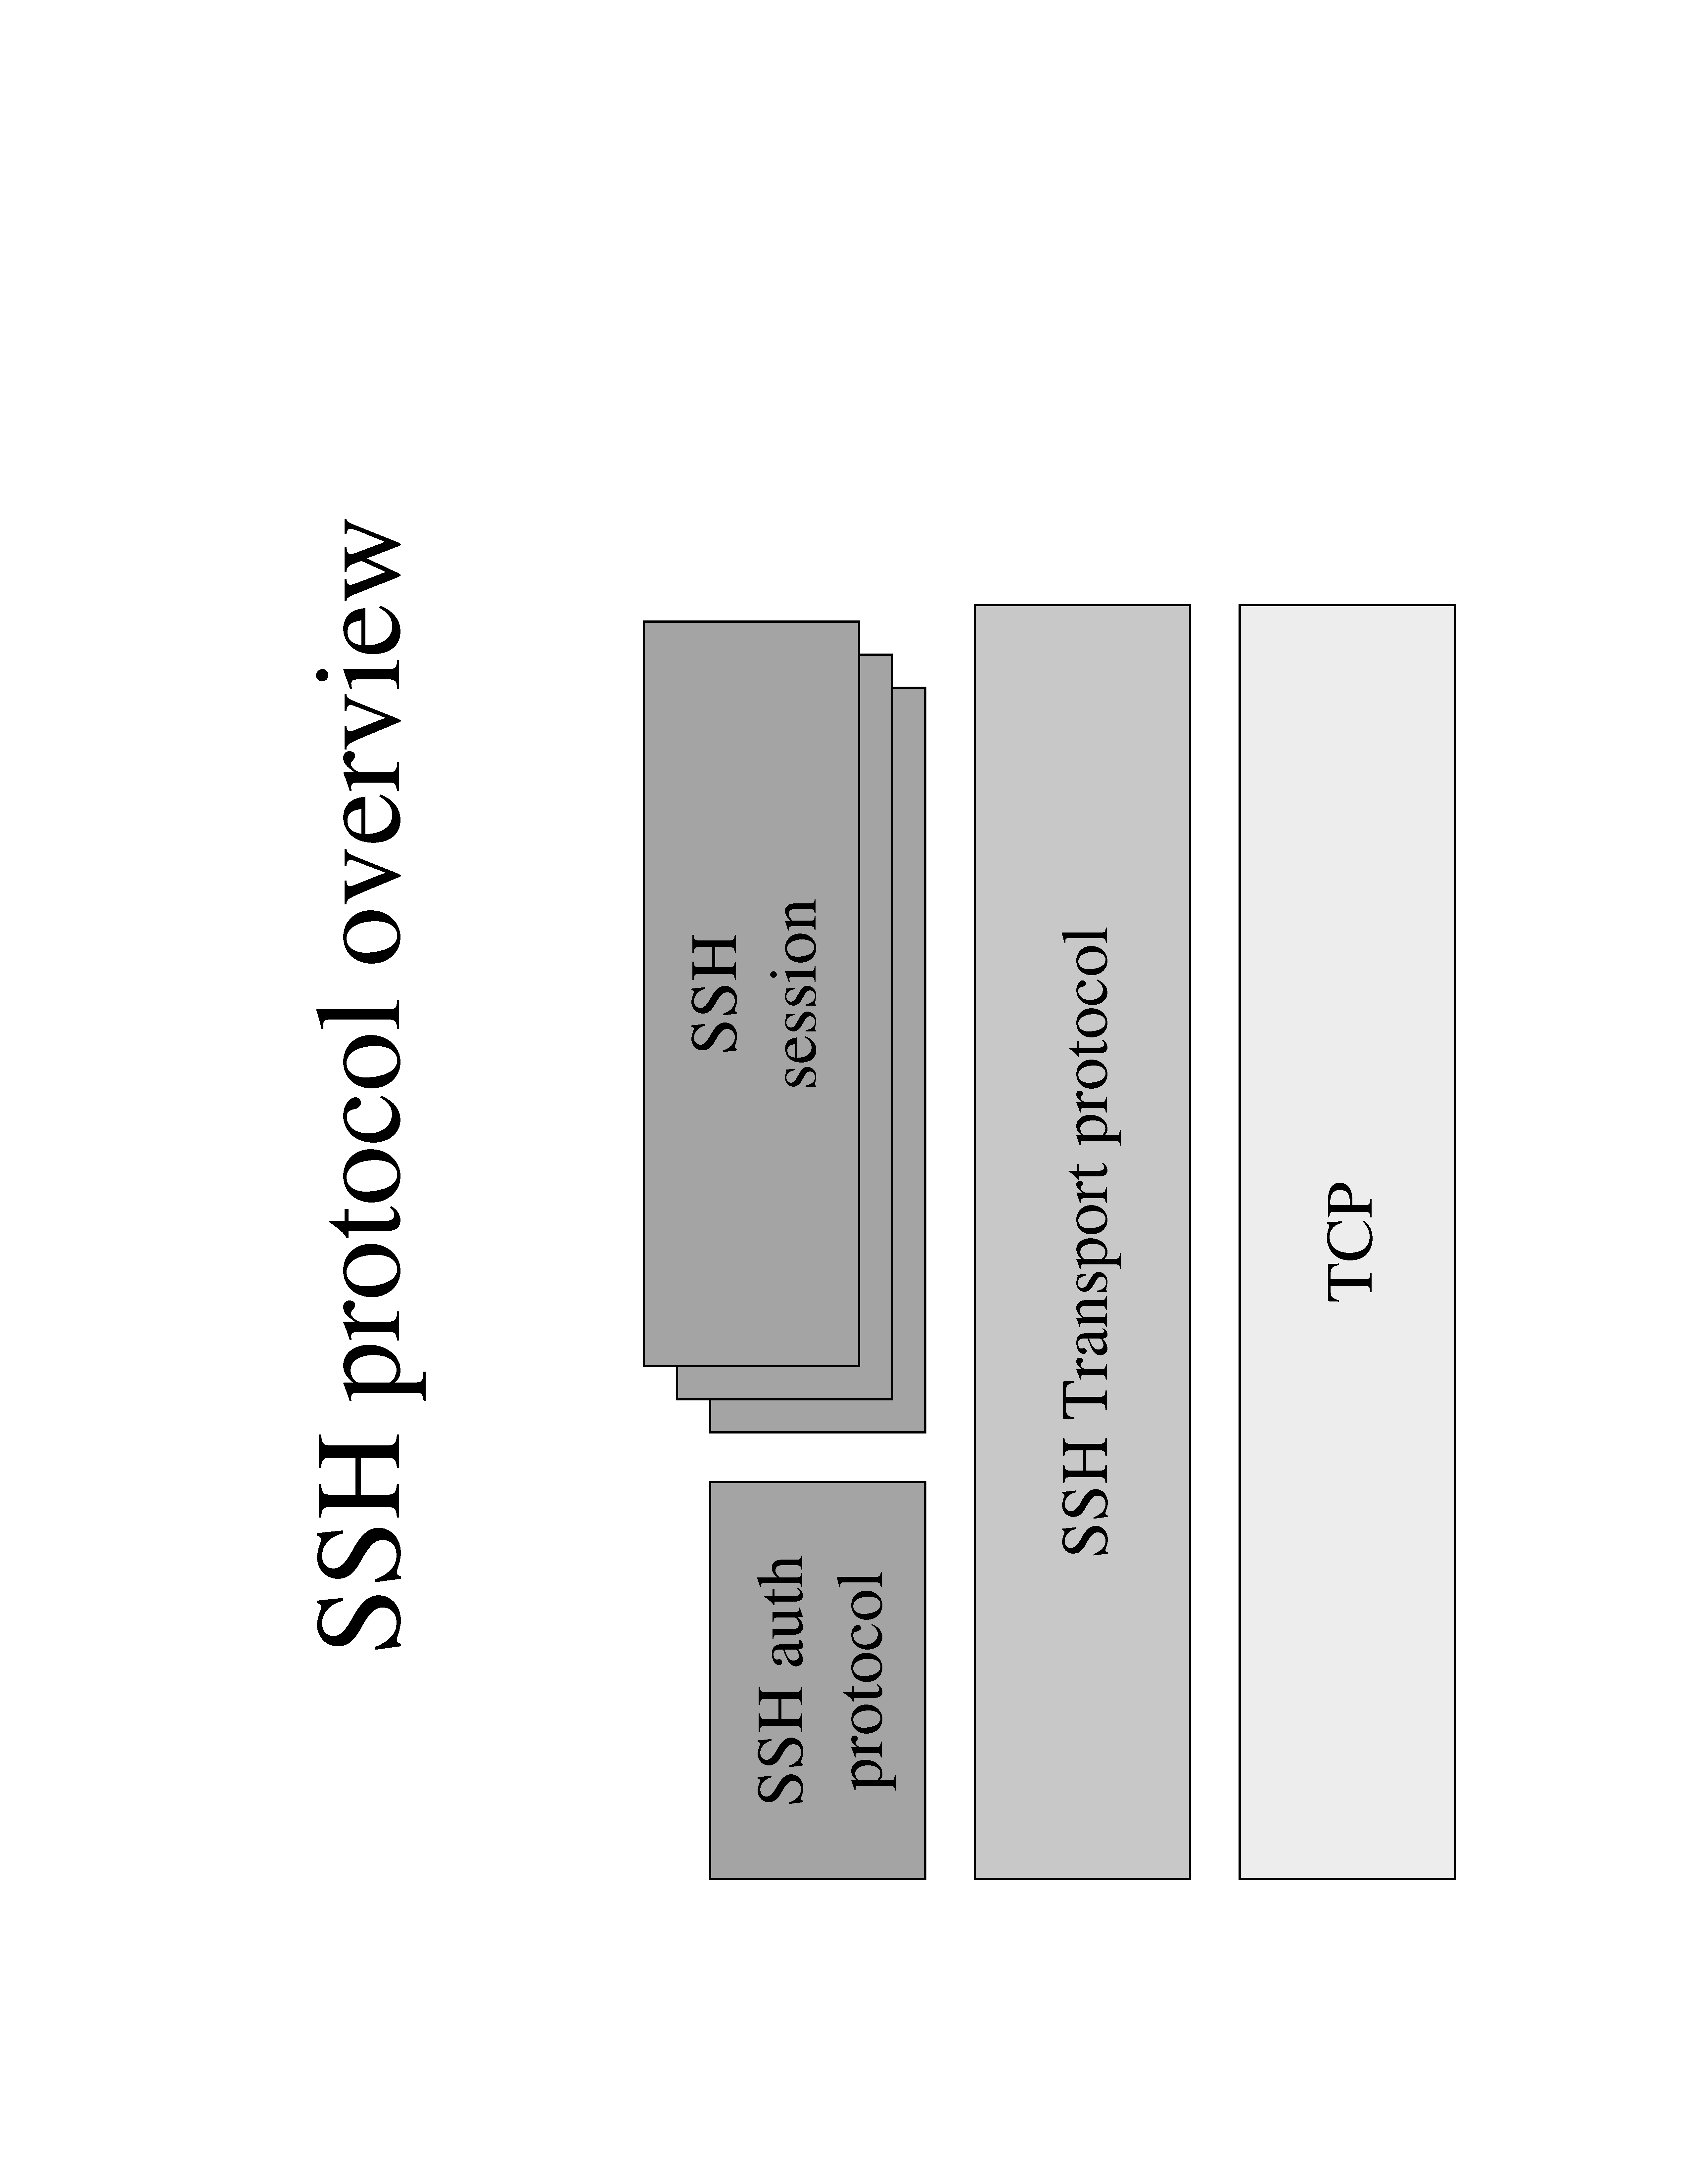
\includegraphics[clip,scale=0.4,angle=270]{ssh_overview}

\caption{\label{fig:ssh-overview} protocol hierarchy}

\end{figure}



\subsubsection{Session Initialization}

The initial handshake provides the client and server with an
opportunity to \textit{1)} perform a key exchange, \textit{(2)}
validate the server key, and \textit{(3)} negotiate an initial set of
cryptographic algorithms that will be used for the session (e.g. for
cipher, HMAC). An overview of the handshake messages are shown in
\ref{fig:ssh-init}. The steps of the protocol are as follows.  Refer
to Figure \ref{fig:ssh2-init} for details.
\begin{enumerate}
\item The SSH server sends a string of the form
  {}``SSH-2.0-\emph{software}''.  The \emph{software} string
  identifies the particular client or server.  (as a variation, it may
  also send SSH-1.99-\emph{software''} to indicate protocol version 1
  compatibility) For example, the OpenSSH 4.5 software sends
  {}``SSH-1.99-OpenSSH\_4.5''. If the client does not understand the
  protocol version, it disconnects, otherwise it sends a similar
  string to the server. After these strings are sent, all traffic uses
  the binary packet protocol shown in Figure \ref{fig:ssh-packet}.\\
%
\begin{figure}
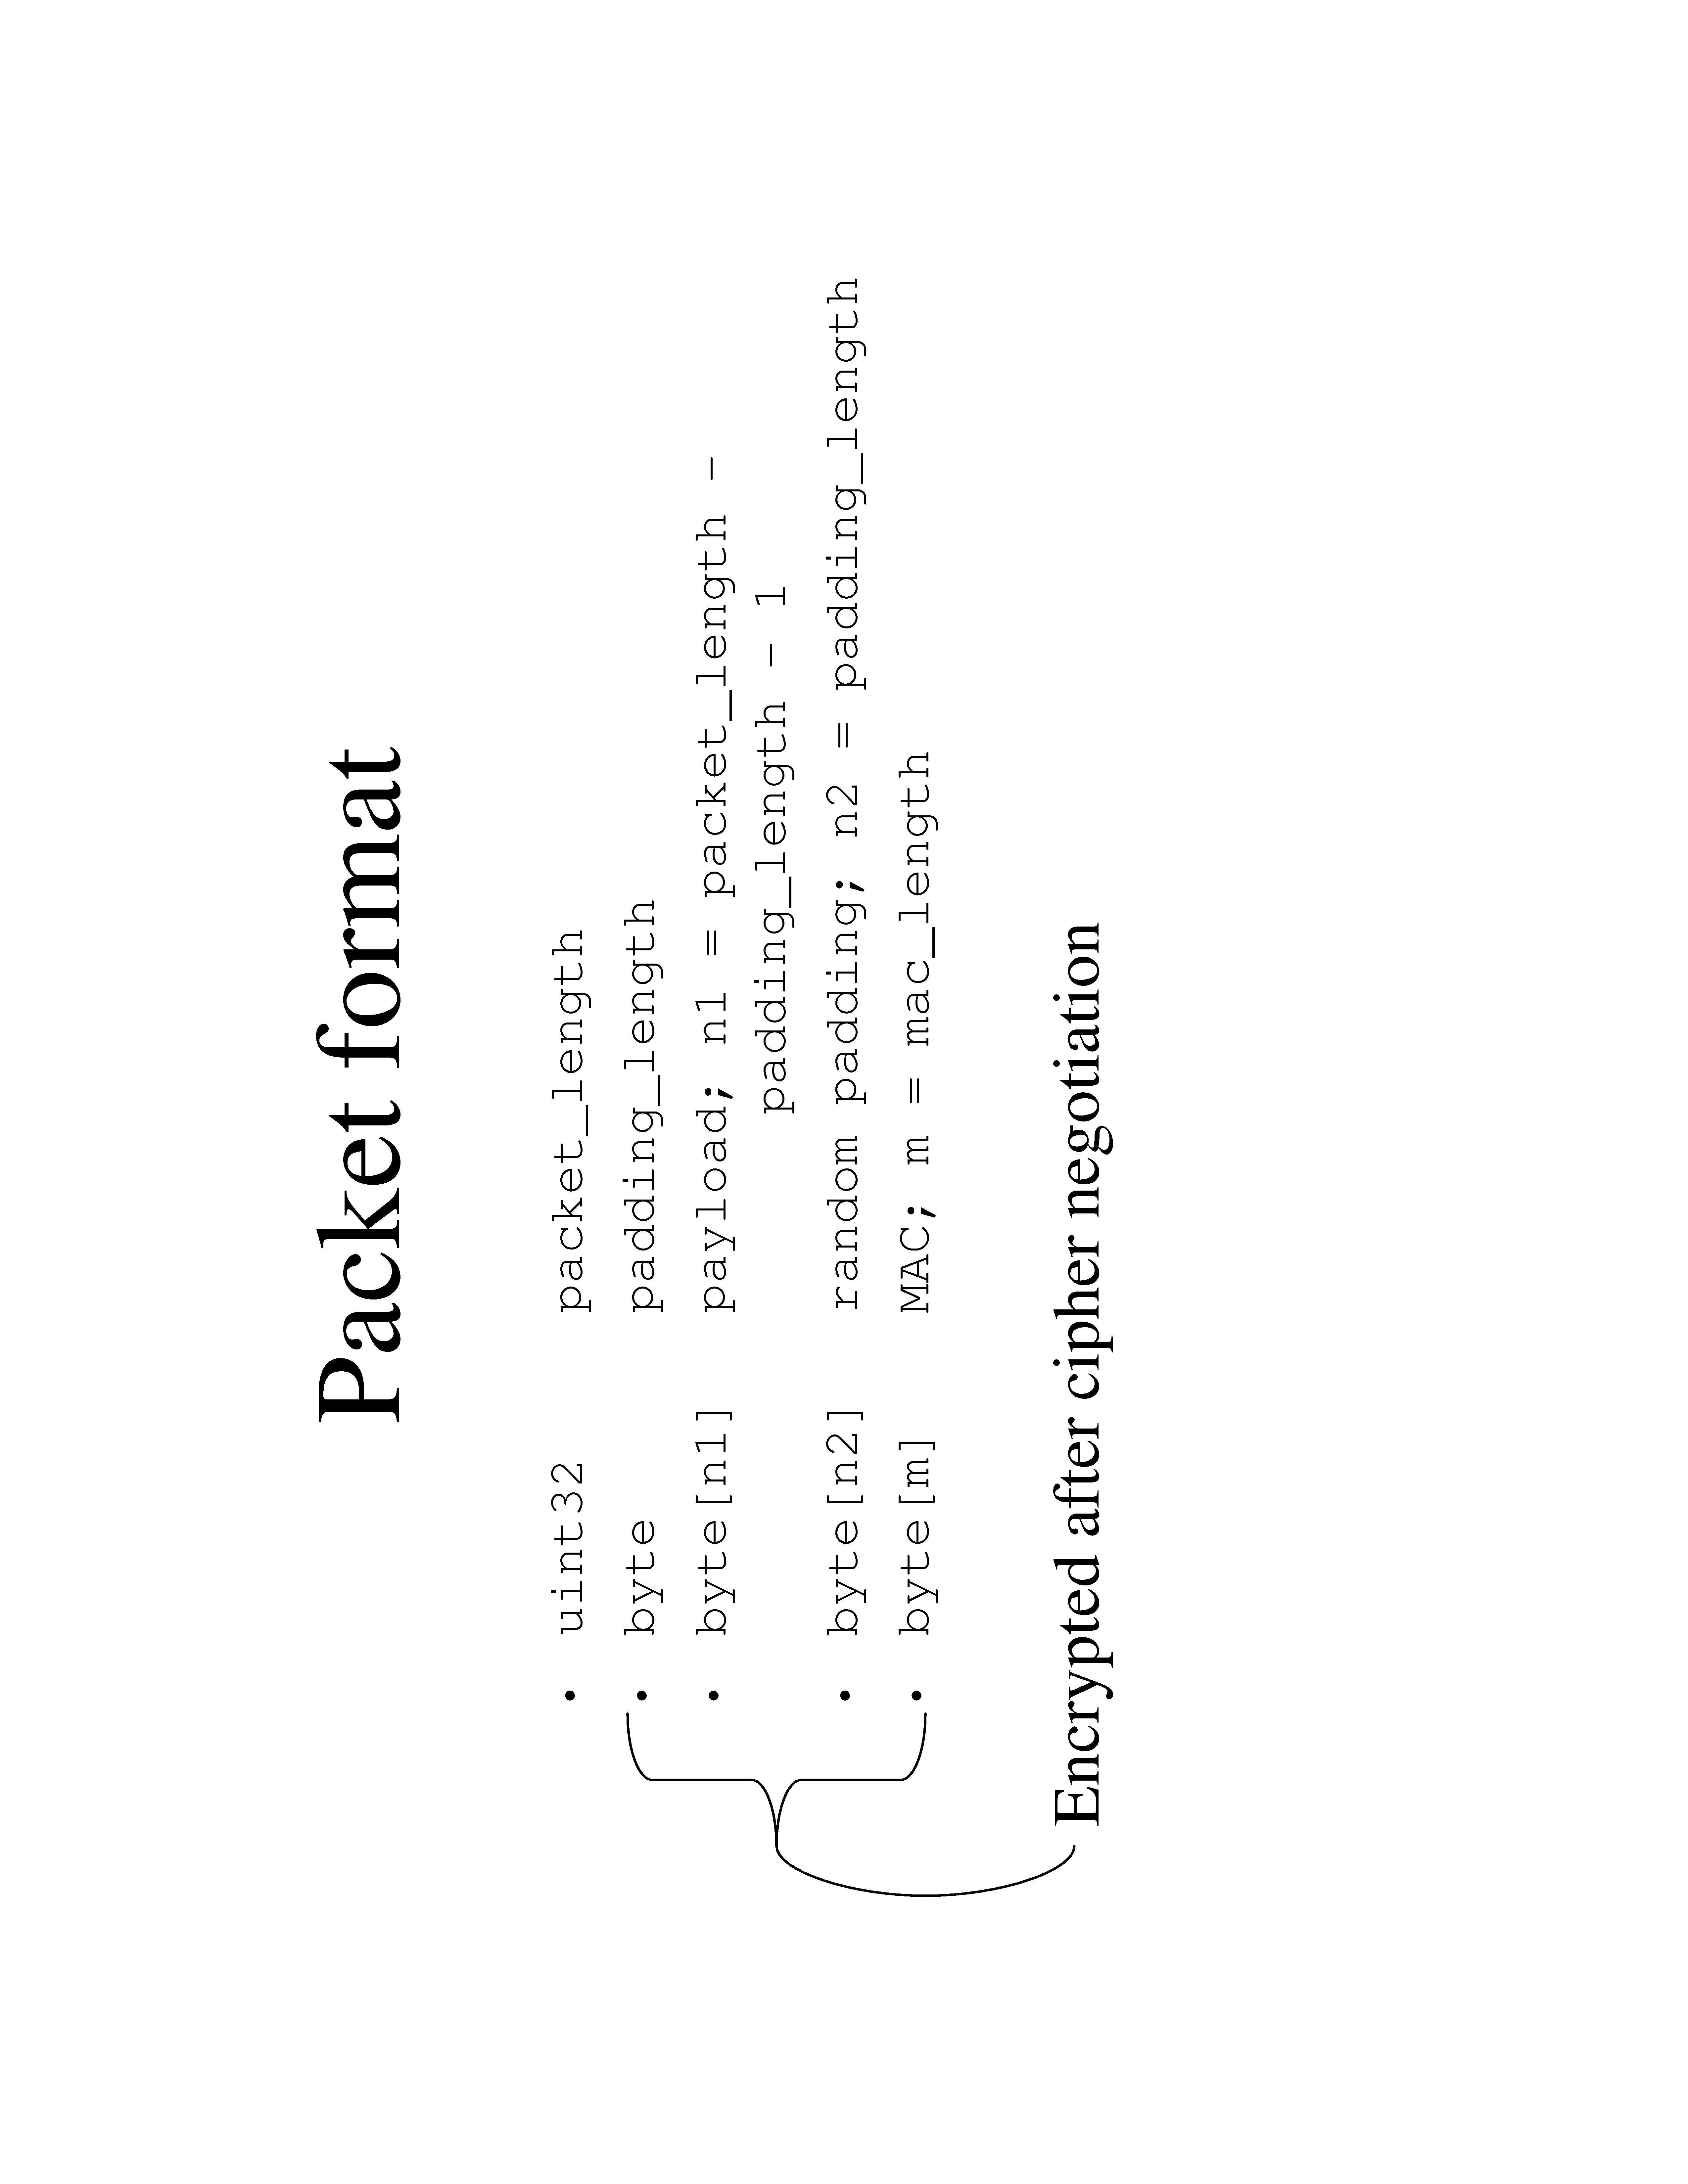
\includegraphics[clip,scale=0.4,angle=270]{ssh_packet}

\caption{\label{fig:ssh-packet} binary packet structure}

\end{figure}

\item Each party sends an SSH\_MSG\_KEXINIT message to begin the key exchange.
This message includes a list of supported ciphers, HMAC algorithms,
compression algorithms, and key exchange algorithms, ranked by preference.
For each algorithm, the parties choose the highest preference algorithm
of the client, which is also supported by the server. If one of the
algorithm lists has no algorithm in common, the connection is terminated.
%% The format of the SSH\_MSG\_KEXINIT message are as follows:

%% \begin{lyxcode}
%% ~~~~~~byte~~~~~~~~~SSH\_MSG\_KEXINIT

%% ~~~~~~byte{[}16{]}~~~~~cookie~(random~bytes)

%% ~~~~~~name-list~~~~kex\_algorithms

%% ~~~~~~name-list~~~~server\_host\_key\_algorithms

%% ~~~~~~name-list~~~~encryption\_algorithms\_client\_to\_server

%% ~~~~~~name-list~~~~encryption\_algorithms\_server\_to\_client

%% ~~~~~~name-list~~~~mac\_algorithms\_client\_to\_server

%% ~~~~~~name-list~~~~mac\_algorithms\_server\_to\_client

%% ~~~~~~name-list~~~~compression\_algorithms\_client\_to\_server

%% ~~~~~~name-list~~~~compression\_algorithms\_server\_to\_client

%% ~~~~~~name-list~~~~languages\_client\_to\_server

%% ~~~~~~name-list~~~~languages\_server\_to\_client

%% ~~~~~~boolean~~~~~~first\_kex\_packet\_follows

%% ~~~~~~uint32~~~~~~~0~(reserved~for~future~extension)
%% \end{lyxcode}
%
\begin{figure}
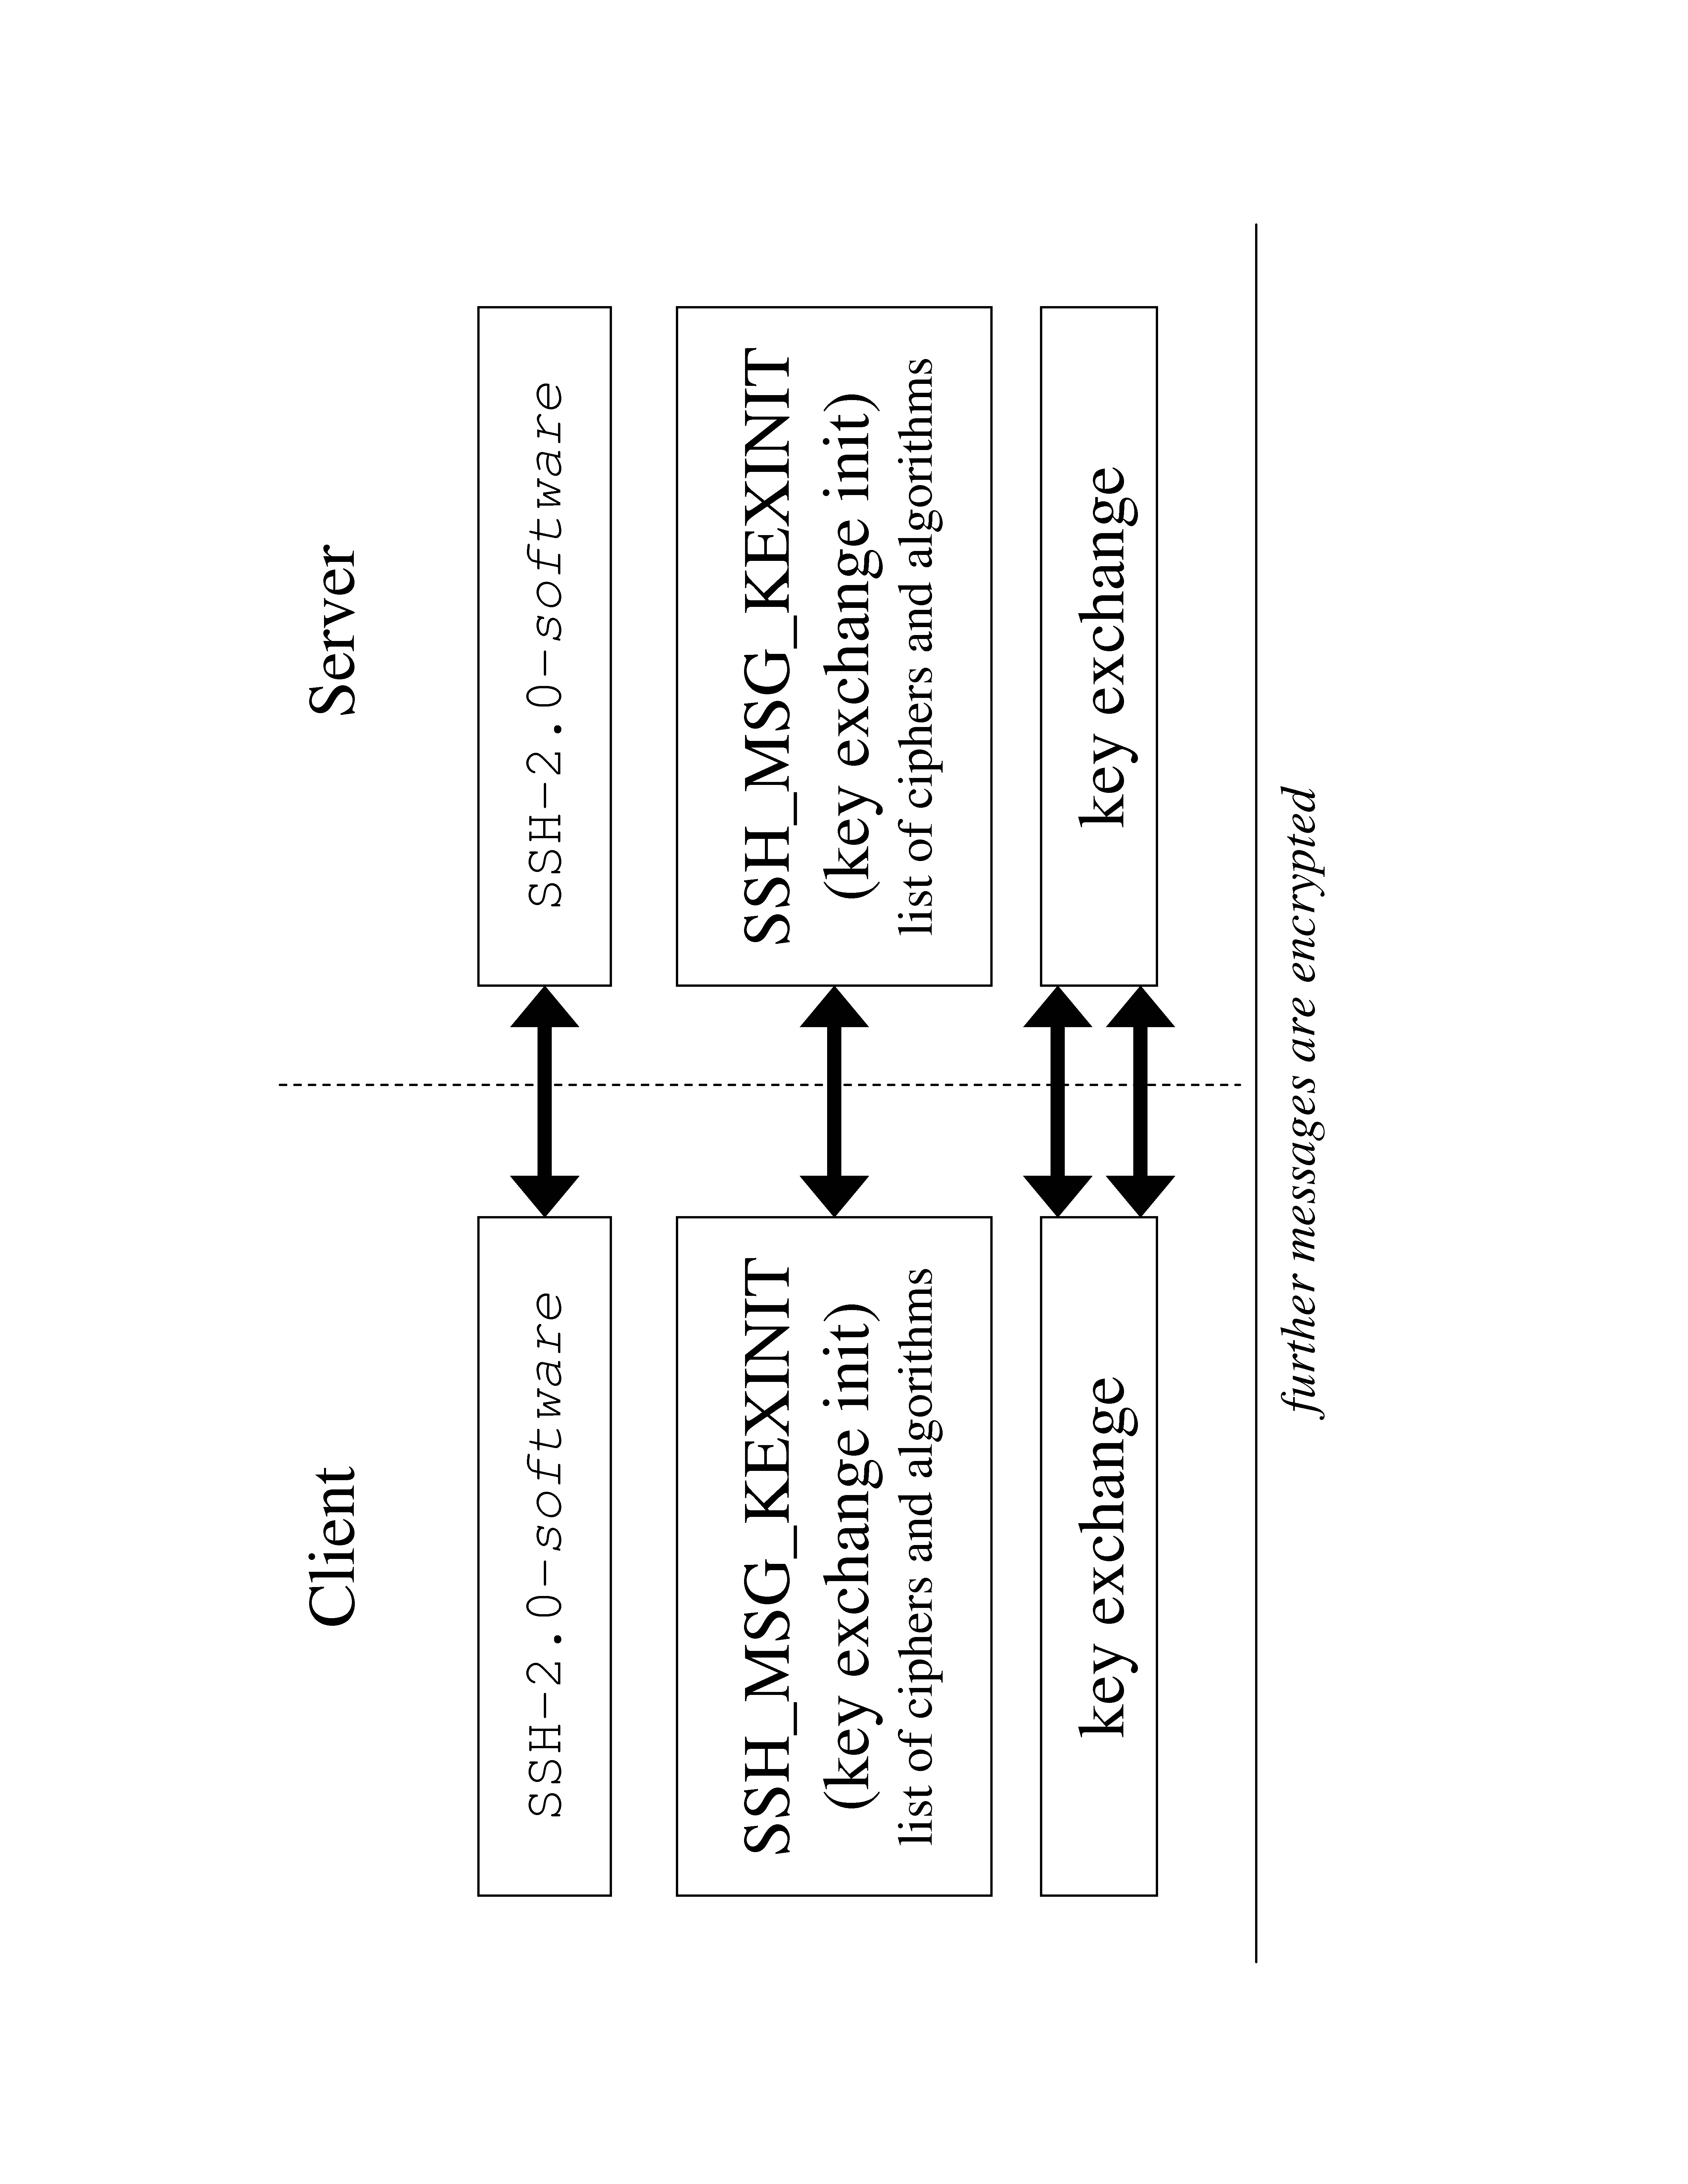
\includegraphics[clip,scale=0.4,angle=270]{ssh_init}

\caption{\label{fig:ssh-init} connection handshake protocol}

\end{figure}


%
\begin{figure}[t]
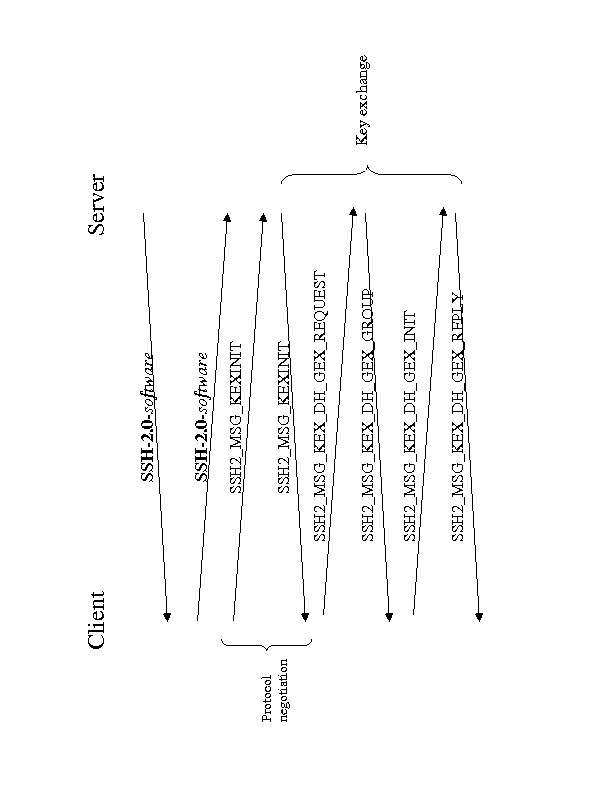
\includegraphics[clip,scale=0.4,angle=270]{ssh2_p1}

\caption{\label{fig:ssh2-init} connection handshake protocol}

\end{figure}


\item Following the handshake, the key exchange protocol is performed. The
specific algorithm used to do the key exchange is negotiated in the
previous step. The original SSH2 specification included a single Diffie-Hellman
group defined in \cite{rfc4253}. A newer and more flexible key exchange
algorithm is defined in \cite{rfc4419}. The details of key exchange
will not be discussed further. After the key exchange is complete,
all of the data in the SSH stream is encrypted using the negotiated
cipher and key. Specifically, the sequence of packets, excluding the
packet size header, shown in \ref{fig:ssh-packet} is a single stream
of plaintext encrypted by the cipher.
\end{enumerate}
At this point, the protocol handshake is complete and the client may
initiate arbitrary sub-protocols of SSH. Typically, the client will
begin the client authentication protocol, as most servers require
authentication before allowing other services to be used.


\subsubsection{Client Authentication}

When the initial handshake is complete, the client has verified the
server key, if possible, but the client has not yet authenticated to
the server. The SSH auth protocol~\cite{rfc4252} can be initiated to
perform this. The auth protocol is flexible; the SSH standard
describes several commonly-used methods of authentication, such as
password and public-key, but arbitrary authentication methods can be
added. The client selects the desired method of authentication among
those supported by the server.

The messages used in password authentication are shown in
\ref{fig:ssh-auth}.  For the purposes of this discussion, we will
assume the client is using the {}``password'' authentication
method. The steps of this authentication are as follows:
\begin{enumerate}
\item The client sends the username and password to the server in an
  SSH\_MSG\_USERAUTH\_REQUEST message. 

%% The format of this message is:

%% \begin{lyxcode}
%% ~~~~~~byte~~~~~~SSH\_MSG\_USERAUTH\_REQUEST

%% ~~~~~~string~~~~user~name~in~ISO-10646~UTF-8~encoding~{[}RFC3629{]}

%% ~~~~~~string~~~~\textquotedbl{}password\textquotedbl{}

%% ~~~~~~boolean~~~FALSE

%% ~~~~~~string~~~~plaintext~password~in~ISO-10646~UTF-8~encoding~


%% \end{lyxcode}
\item If the server does not support the {}``password'' method chosen,
or the password is incorrect, the server will respond with an SSH\_MSG\_USERAUTH\_FAILURE
message. If the password is correct, the server sends a SSH\_MSG\_USERAUTH\_SUCCESS
message, and the client may begin requesting services. (The server
may also send a SSH\_MSG\_USERAUTH\_BANNER packet to communicate information
directly to the user. It is analogous to the /etc/issue file used
in standard Unix systems to display a message at a login prompt)
\end{enumerate}
%
\begin{figure}
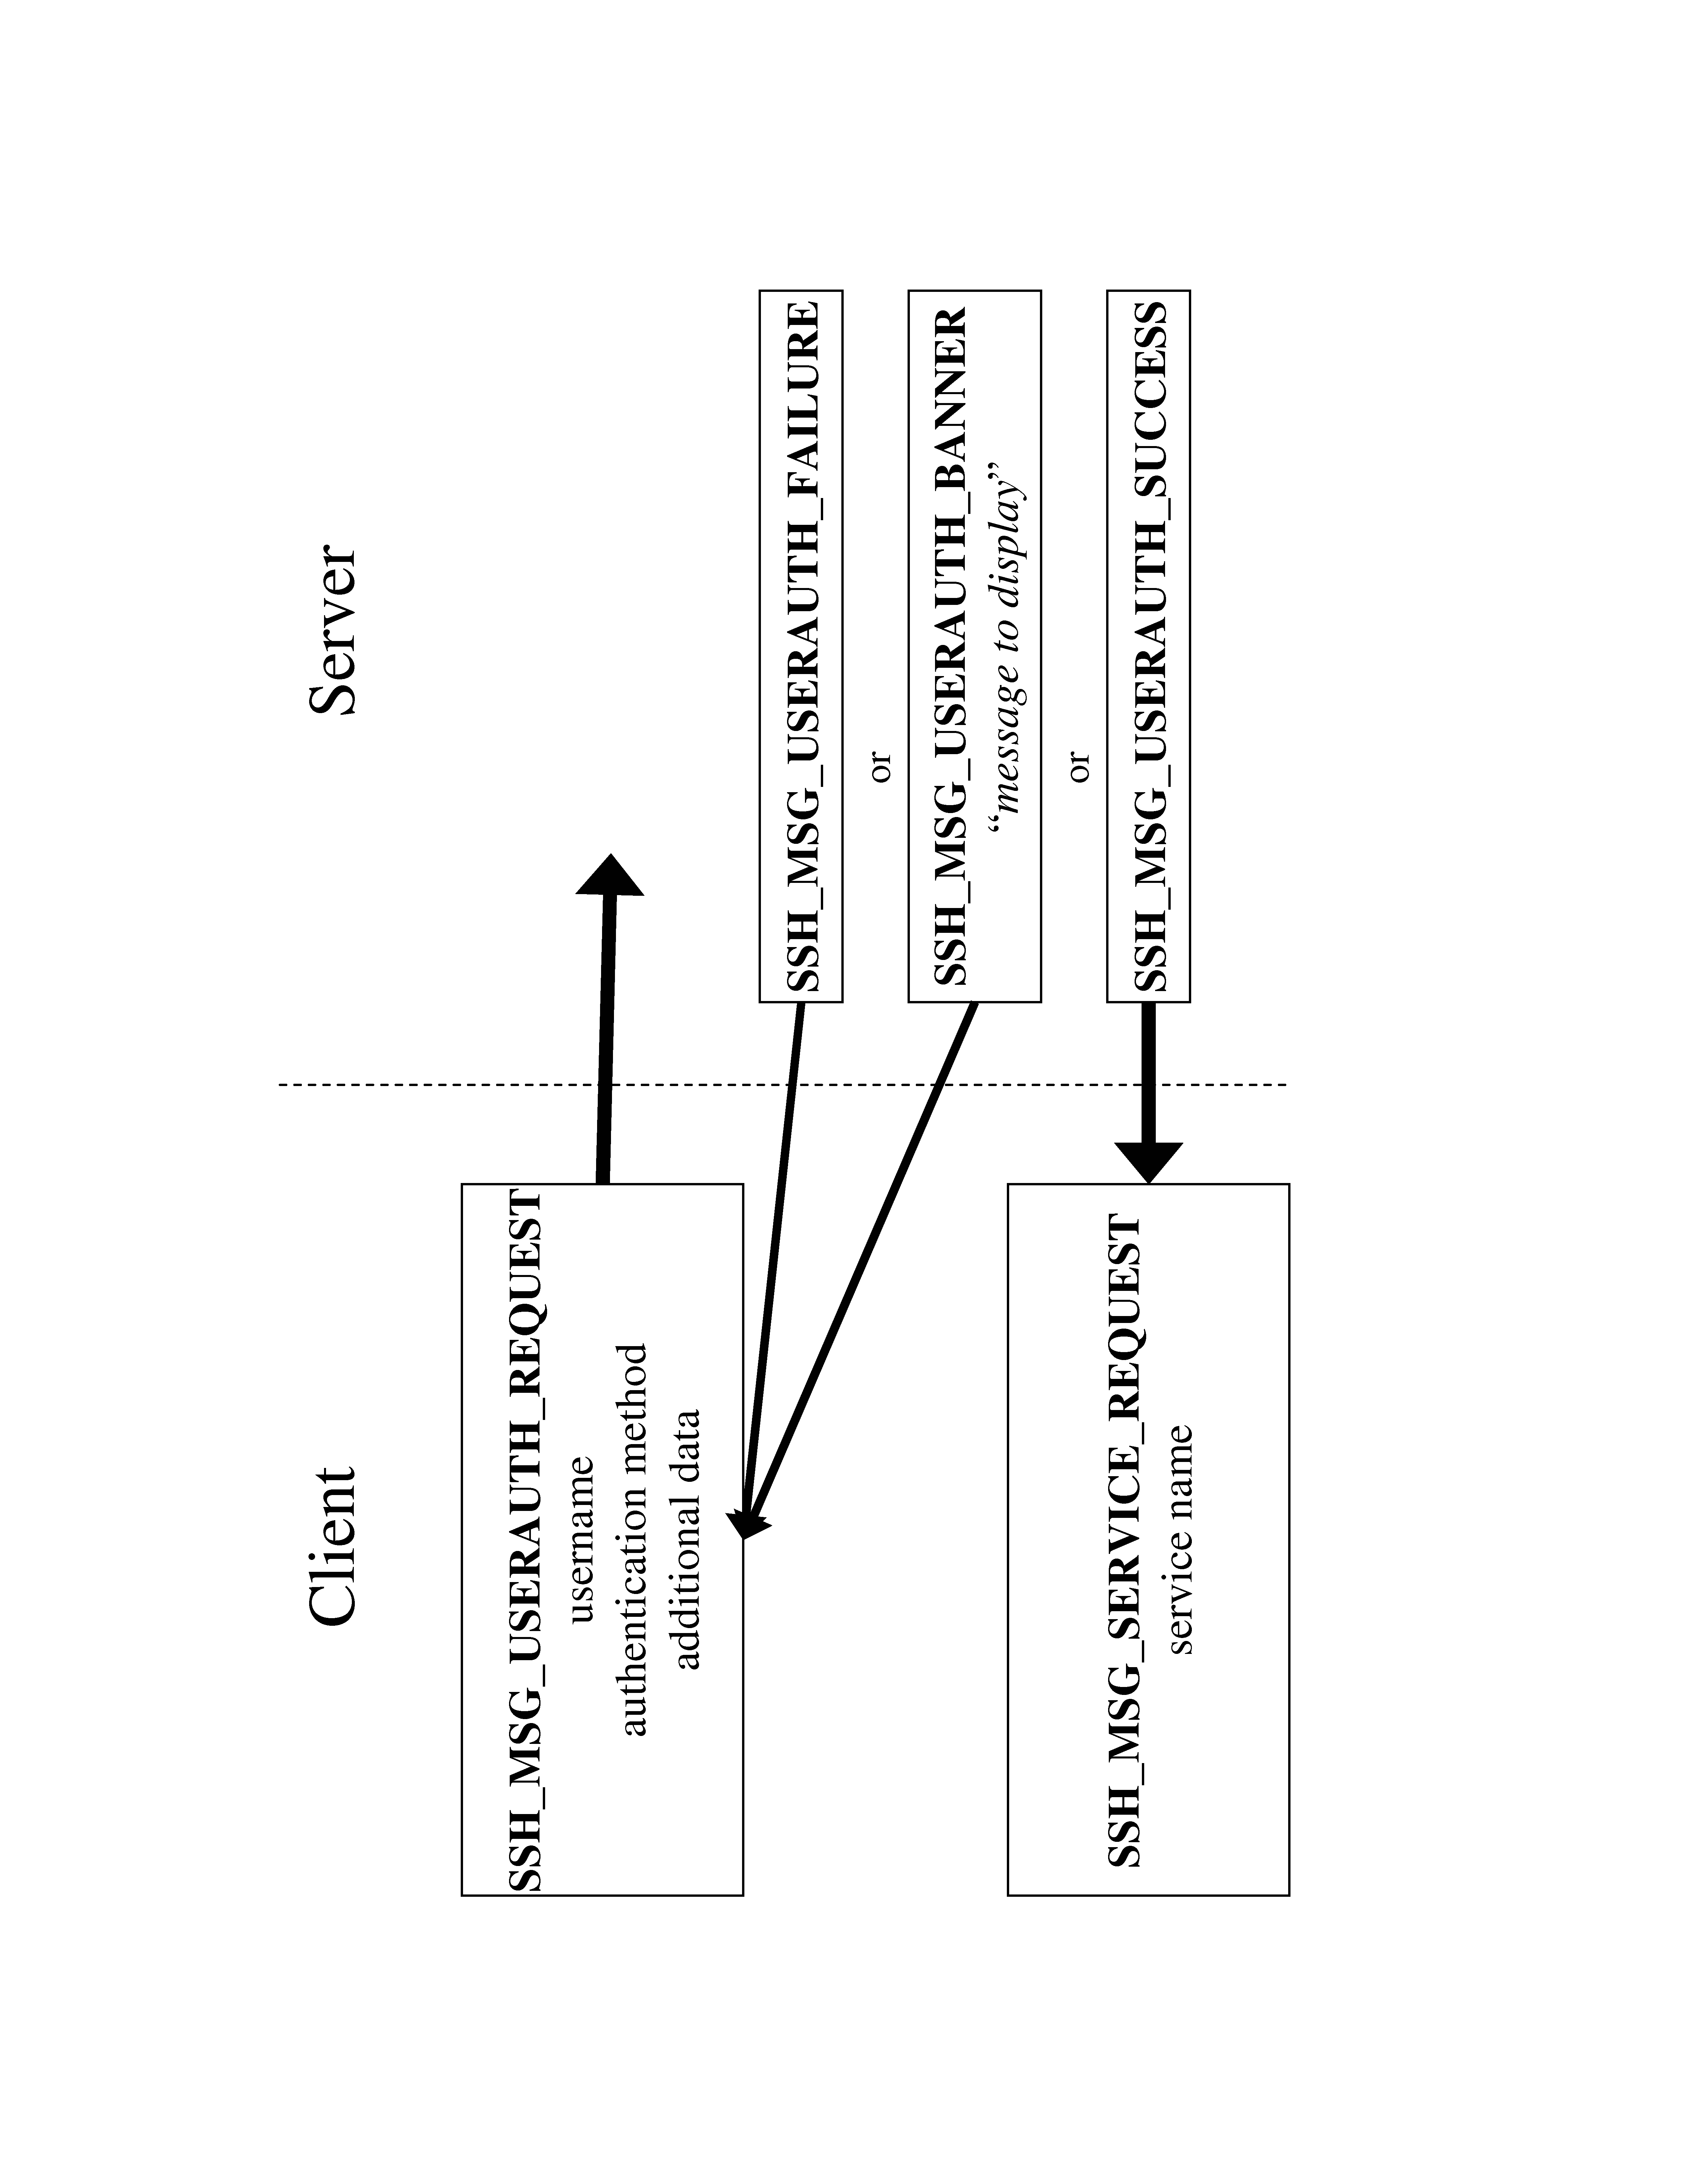
\includegraphics[clip,scale=0.4,angle=270]{ssh_auth}

\caption{\label{fig:ssh-auth} authentication protocol messages}

\end{figure}


The password is sent directly from the client to the server in a
packet. Thus, the only protection from eavesdroppers is the encryption
applied at the SSH transport layer. There is no protection of the
client's authentication credentials from the server itself, so if the
server is malicious or has been compromised, an attacker will learn
everything the client sends, and can potentially impersonate the
client at another time.


\subsection{Man in the Middle Attack}

As mentioned in the overview, as well as the previous section, the SSH
protocol is vulnerable to password compromise. An attacker can exploit
the insecurity of password transmission by mounting a \emph{man in the
  middle} (MITM) attack. Although the protocol does provide some
protection against MITM in the form of host key authentication, there
are several ways in which an attacker can thrwart this protection:
\begin{enumerate}
\item If the attacker manages to steal the host key, then the attacker can
successfully impersonate the server without detection. There is no
other means for the client to authenticate the server.
\item If the client does not know the server's host key, then the host
  cannot be authenticated unless the client has an alternative trusted
  channel to validate the host key. As mentioned in the overview, the
  following message is typically displayed by the OpenSSH client when
  connecting to a server with an unknown key\\
%
\begin{minipage}[t]{1\columnwidth}%
\begin{lyxcode}


The~authenticity~of~host~'server~(1.2.3.4)'~can't~be~established.

RSA~key~fingerprint~is~3f:76:22:43:c2:03:b9:71:b0:31:ce:87:37:45:cb:02.~

Are~you~sure~you~want~to~continue~connecting~(yes/no)?
\end{lyxcode}
%
\end{minipage}\\

Practically speaking, it may be inconvenient for a user to authenticate
the server using this message and make a correct decision. It is easy
to imagine a user simply answering yes in order to bypass the inconvenience. 
\item Even if the client does know the server's key, the there is no
  guarantee that a user would refuse to connect even if the
  authentication fails. In fact, there are several reasonable
  explanations for why a user may choose to accept a failed
  authentication and continue with the connection. For example, the
  user might think the server key changed for a non-malicious reason
  such as an operating system upgrade where the administrator forgot
  to backup the old key.
\end{enumerate}

While the only method that guarantees the success of the attacker is
\textit{(1)}, each poses a real security problem for users of SSH.

\subsection{SPAKA using SFE}

As previously hinted, this vulnerability can be mitigated by using
additional secrets which are shared between the client and server. The
password is a convenient shared secret already in common use
today. Typically, a password is considered only as a means of
authenticating a client to a server, but with certain protocols a
password can also be used for simultaneous mutual authentication in a
way that is secure, and does not compromise the password if the server
is malicious. Such protocols are known as \emph{secure password and
  key authentication} (SPAKA).

It is important to note that a {}``password'' need not be a constant
string that the user remembers over a long period of time, it can be
any string that serves as a mutual authenticator. For example, secure
ID tokens that display constantly changing strings, time synchronized
with the server, are considered to be a more secure alternative to
traditional passwords, such alternatives are readily usable in SPAKA
protocols.

The design of previous SPAKA protocols~\cite{brainard03} suggests that
SFE can be applied generally to the SPAKA problem. Here is a general
SPAKA construction based on SFE:

\begin{enumerate}

\item Let $X$ be the user's password, $Y=H(X)$ be a hash of $X$.

\item Let $C$ be the client and $S$ be the server. $C$ and $S$ participate
in a secure evaluation of the following function $f$, where $C$
provides input $X$ and $S$ provides input $Y$. $C$ and $S$ both
receive the same output from $f$, which is a single bit denoting a
boolean value.
\[
f(X,Y)=_{def} \left(Y=H\left(X\right)\right)
\]
If the value of the $f$ is $false$ then it is evident that one of the
parties did not possess the shared secret, and the mutual
authentication fails. Otherwise the mutual authentication succeeds.

\end{enumerate}

Notice that $f$ is nothing more than a variant of the well-known
millionaire problem, where the relational predicate used is equality
rather than less than or greater than. If $f$ is evaluated securely,
then $C$ and $S$ are guaranteed not to learn any information about the
computation except for the single bit of output, thus allowing them
mutual authentication without revealing any information to potential
attackers. This authentication scheme can be integrated into
implementations of the SSH protocol trivially to provide protection
from the MITM attack previously described.

%
\begin{comment}
\begin{enumerate}
\item Practical SSH paper
\item New protocol paper
\item Theoretical paper
\item Graduate!!!
\end{enumerate}

\end{comment}
{}


\section{Implementation}

We implemented an SSH client and server that incorporate this SPAKA
protocol. The following components were used:
\begin{enumerate}
\item The Dropbear SSH client and server. We chose to use this client
because of it's small and simple codebase.
\item The SFE-Tools secure function evaluation compiler first described
by Kruger \textit{et al.}
\end{enumerate}
A new authentication method was defined in the client and server code
using the extensible SSH architecture. To initiate the SPAKA
authentication protocol, the client sends an authorization protocol
request:
\begin{lyxcode}
~~~~~~byte~~~~~~SSH\_MSG\_USERAUTH\_REQUEST

~~~~~~string~~~~username

~~~~~~string~~~~\textquotedbl{}sfeauth\textquotedbl{}

~~~~~~boolean~~~FALSE
\end{lyxcode}
The server responds with the type of password hashing used to store
passwords on this system. Examples include {}``DES'' for the traditional
UNIX password crypt function, and {}``MD5'' for the default password
hashing algorithm used on most modern Linux systems. 
\begin{lyxcode}
~~~~~~byte~~~~~~SSH\_MSG\_USERAUTH\_RESPONSE

~~~~~~string~~~~username

~~~~~~string~~~~\textquotedbl{}MD5\textquotedbl{}

~~~~~~boolean~~~FALSE
\end{lyxcode}
After this exchange, the client prepares an encrypted circuit corresponding
to the hashing method in use. The underlying SFE protocol runs, wrapped
inside SSH messages SSH\_MSG\_USERAUTH\_MSG1 and SSH\_MSG\_USERAUTH\_MSG2.

\section{Related Work}

\subsection{SPAKA}

\emph{Secure Password and Key Authentication} (SPAKA) is a class of
authentication protocols first described in \cite{bellovin92}. SPAKA
protocols are designed to guarentee confidentiality of secrets even
against active adversaries. There have been various SPAKA protocols
proposed in the literature with varying properties. A recent SPAKA
protocol is presented in \cite{brainard03}. In this protocol, the
user's password $P$ is split into two shares: $P_{1}$ and $P_{2}$.
The value of $P$ can not be derived from either of the two shares
alone, and each share is stored on a seperate server. To perform the
protocol, the client splits $P$ into different shares $P_{1}'$ and
$P_{2}'$, and sends these values to the servers. The servers then
perform an evaluation protocol to determine if $P_{1}\oplus P_{2}=P_{1}'\oplus P_{2}'$.

\bibliographystyle{plain}
\bibliography{somesh,ssh}

\end{document}



\part{Timeline}


\subsection{Summer 2007}
\begin{itemize}
\item Secure authentication in SSH (see section \ref{sub:SPAKA-using-SFE})

\begin{itemize}
\item define protocol extension
\item implement classic SPAKA 
\item implement SFE SPAKA
\item benchmark and compare
\end{itemize}
\item Target publication: Usenix Security 2008
\end{itemize}

\subsection{Fall 2007}
\begin{itemize}
\item Investigate optimizations of cryptographic primitives (see section
\ref{sub:Other-Optimizations})

\begin{itemize}
\item adapt standard oblivious transfer algorithms to use more efficient
representations, such as elliptic curve groups
\item evaluate modular square root oblivious transfer (see section \ref{sec:OT-SquareRoots})
\item investigate use of other kinds of functions for oblivious transfers
and homomorphic encryption
\end{itemize}
\item Target publication: TBD
\end{itemize}

\subsection{Winter/Spring 2008}
\begin{itemize}
\item Investigate use of other circuit representations (see section \ref{OBDD-section})

\begin{itemize}
\item evaluate which OBDD extensions are good candidates for secure protocols
\item implement compiler and protocols
\item performance measurements
\end{itemize}
\item Target publication: TBD
\end{itemize}

\subsection{Spring/Summer 2008}
\begin{itemize}
\item Investigate optimizations resulting from controlled leakage of information.
(see section \ref{sub:Other-Optimizations})

\begin{itemize}
\item Develop specification language to tag intermediate values as sensitive
or non-sensitive
\item Develop hybrid evaluation protocols that protect sensitive data but
avoid the overhead when evaluating non-sensitive computations
\item Implement and measure performance gains
\end{itemize}
\end{itemize}

\subsection{Fall/Winter 2008}
\begin{itemize}
\item Optimizing protocol compiler. (see section \ref{sub:An-Efficient-Framework})

\begin{itemize}
\item Define programming language for expressing secure computations

\begin{itemize}
\item Language will include direct support for common SFE techniques, such
as homomorphic encryption, and metadata for privacy levels
\end{itemize}
\item Implement compiler for this language into securely evaluable {}``machine
code''
\item Automatic optimizer will try different representations of the functions,
including OBDDs, Boolean circuits, and other ideas from my research,
and produce as efficient as a representation as possible
\item Implement protocol evaluation library, to make straightforward use
in ordinary applications.
\end{itemize}
\end{itemize}

\subsection{Spring 2009}
\begin{itemize}
\item Write dissertation and graduate.
\end{itemize}



\bibliographystyle{plain}
\bibliography{privacy,somesh,ssh,crypto}

\end{document}
